\documentclass[a4paper,12pt,openright,notitlepage,twoside]{book}
\raggedbottom % lascia alla fine delle pagine lo spazio invece che adattarle


% pacchetti da caricare
\usepackage[table]{xcolor}
\usepackage[T1]{fontenc} % definisce i caratteri di output
\usepackage{afterpage}
\usepackage[utf8]{inputenc} % definisce i caratteri di input
\usepackage[italian,english]{babel} % definisce la lingua del documento
\usepackage[headheight=15pt]{geometry} % definisce i margini del documento
\geometry{a4paper,top=30mm,bottom=30mm,left=30mm,right=25mm,heightrounded,bindingoffset=3mm}
\usepackage{fancyhdr} % serve per gestire intestazione e piè di pagina
\pagestyle{fancy}
\usepackage{emptypage} % serve per fare le pagine vuote
\usepackage[pdftex]{hyperref} % serve per ottenere links e indice cliccabili
\hypersetup{colorlinks=true,allcolors=black}
\usepackage{microtype} % migliora la scrittura del testo
\usepackage{appendix} % serve per personalizzare l'appendice
\usepackage[printonlyused]{acronym} % serve per creare l'elenco degli acronimi
\usepackage{eurosym} % serve per scrivere il singolo dell'euro
\usepackage{siunitx} % serve per mettere le unita` di misura nel SI
\usepackage{mathtools} % serve per fare le formule matematiche (carica anche AMSMATH)
\usepackage{booktabs} % serve per fare le tabelle più belle
\usepackage{multirow} % serve per fare le tabelle con righe complesse
\usepackage{pgfplotstable} % serve per fare tabelle da file con dati tabulati
\usepackage{graphicx} % serve per fare le figure
\usepackage{tikz} % serve per fare i grafici
\usepackage{pgfplots} % serve a fare i grafici anche lui
\pgfplotsset{compat=1.14}
\usepackage{subcaption} % serve per aggiungere la didascalia alle figure composte (carica anche CAPTION)
\captionsetup{font=small,labelsep=colon}
\usepackage{tocloft} % serve per fare le liste di figure e tabelle più belle
%\usepackage{cite} % serve per mettere le citazioni bibliografiche
\usepackage{biblatex} %serve per la bibliografia
\addbibresource{references.bib}
%\usepackage{eurosym}
%\usepackage{mathabx}
\usepackage{amsmath,amssymb}
\usepackage{tabularx}
\usepackage{setspace}
\usepackage{amsmath}


% modifiche dei comandi
\renewcommand{\chaptermark}[1]{\markboth{\chaptername\ \thechapter.\ #1}{}} % modifica l'intestazione con il nome/numero del capitolo
\renewcommand{\sectionmark}[1]{\markright{\thesection.\ #1}} % modifica l'intestazione con il nome/numero dela sezione
\renewcommand{\cftfigfont}{Figure } % per aggiungere "Figure " nella lista delle figure
\renewcommand{\cfttabfont}{Table } % per aggiungere "Table " nella lista delle tabelle
\newcommand{\omissis}{[\textellipsis\unkern]}


% dichiarazioni personalizzate
\DeclarePairedDelimiter{\abs}{\lvert}{\rvert} % per fare il valore assoluto
\DeclarePairedDelimiter{\norma}{\lVert}{\rVert} % per fare la norma



\begin{document}

%\frontmatter % serve per mettere i numeri romani come numeri di pagina 
\thispagestyle{empty} % serve per rimuovere tutte le impostazioni delle pagine dalla prima pagina

% FRONTESPIZIO
\begin{center}
% Intestazione
\Large{\textbf{Politecnico di Milano}} \\
\vspace{-4mm}
\rule{\textwidth}{0.4pt}
\normalsize{SCHOOL OF INDUSTRIAL AND INFORMATION ENGINEERING} \\
\normalsize{Master of Science -- Computer Science and Engineering} \\
\vspace{20mm}
% Logo Politecnico
\begin{figure}[h!]
\centering
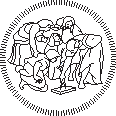
\includegraphics[height=0.20\textheight]{images/logo_poli_bianco}
\end{figure}
\vspace{12mm}
% Titolo Tesi
\huge{\textbf{A Machine Learning approach for automatic disease detection in Chest X-Rays}} \\
\vspace{22mm}
\end{center}

% Relatore/Correlatore
\begin{flushleft}
\normalsize{Supervisor} \\
\small{\textbf{Prof. Pier Luca Lanzi}} \\
\vspace{5mm}
\normalsize{Co-Supervisors} \\
\small{\textbf{Prof. Daniele Loiacono}} \\
\small{\textbf{Dr. Edoardo Giacomello}} \\
\end{flushleft}
\vspace{10mm}

% Autore
\begin{flushright}
\normalsize{Candidate} \\
\small{\textbf{Luca Nassano -- 893812}} \\
\end{flushright}
\vspace{13mm}

% Piè Di Pagina
\begin{center}
\rule{\textwidth}{0.4pt}
\small{\textbf{Academic Year 2018 -- 2019}}
\end{center}


% modifica intestazione e piè di pagina del corpo del documento
\fancyhead{} % cancella tutti i campi dell'intestazione
\fancyfoot{} % cancella tutti i campi del piè di pagina
\fancyhead[LE,RO]{\leftmark}
\fancyfoot[LE,RO]{\thepage}
\renewcommand{\headrulewidth}{0.4pt}
\renewcommand{\footrulewidth}{0pt}


% carico le varie parti della tesi
\chapter*{Ringraziamenti}
\label{cha:ringraziamenti}
\markboth{Acknowledgements}{}
\addcontentsline{toc}{chapter}{Acknowledgements}
\doublespacing
\noindent Un immenso grazie alla mia famiglia. A mamma e papà, per avermi dato l'opportunità di arrivare fino a qui, per avermi spronato ogni giorno a dare il meglio di me e per avermi insegnato tutto, grazie per aver fatto di me la persona che sono oggi. Ai miei fratelli, Andrea e Filippo, per aver condiviso con me me tutti questi anni, fatti di alti e bassi, grazie per esserci sempre stati. Il vostro sostegno è stato fondamentale. Vi voglio bene.

\vspace{5mm}

\noindent A tutte persone che son state vicine a me e alla mia famiglia in questi anni: Gianni, Enrico, Silvio, Francesca e Luisa, non dimenticherò mai il vostro supporto.

\vspace{5mm}

\noindent Ai miei amici. A Emanuel per aver condiviso con me questo viaggio, un traguardo dopo l'altro. A Riccardo, Marco ed Erik, per aver reso indimenticabili questi anni. 

\vspace{5mm}

\noindent Al professor Loiacono, al professor Lanzi e al Dr. Giacomello, per la loro disponibilità e per avermi aiutato, in questi mesi, a portare a termine questo lavoro.

\vspace{5mm}

\noindent A tutte le persone che non ho menzionato ma che mi sono state accanto durante questo percorso, grazie ad ognuno di voi per aver contribuito ad arrivare fino a qui.
\chapter*{Abstract}
\label{cha:abstract}
\markboth{Abstract}{}
\addcontentsline{toc}{chapter}{Abstract}

Chest X-Rays, due to their simplicity and non-invasive nature, are one of the most common tools used for the detection of many diseases. During the last years the scientific community published different datasets containing CXR images, along with side information related to the presence or absence of different pathologies.
This work studies the problem of analyzing them, with the aim of building an automatic system able to check whether a patient suffer from a given disease or not. Moreover, it tries to overcome the so called black-box problem, an issue connected to many machine learning applications, related to the fact that they are able to provide a decision but they’re not capable of giving an explanation behind such decision. This work tries to solve it by producing, along with the prediction, a heatmap highlighting the region that most probably is affected by the disease and a bounding box surrounding it. In particular, in this work we investigate different approaches, ranging from Convolutional Neural Network, widely employed in other related works, to the less used Random Forest, trained using a low dimension representation of the input, the so called embeddings. We also propose a novel technique to combine different predictions, that exploit the uncertainty of the single model to assign it a proper weight during the aggregation phase. Although we weren’t able to surpass the performance of some related works, we obtained a mean AUROC of 0.902 over five different pathologies, showing that good results can be achieved also by models that are computationally more efficient and require much less time to be trained with respect to CNNs.

\chapter*{Estratto in lingua Italiana}
\label{cha:estratto}
\markboth{Estratto}{}
\addcontentsline{toc}{chapter}{Estratto in lingua Italiana}

Le radiografie del torace, data la loro semplicità e natura non invasiva, sono uno degli strumenti più comunemente utilizzati per la rilevazione di molte malattie. Negli ultimi anni la comunità scientifica ha pubblicato diversi dataset contenenti radiografie toraciche, accompagnate da informazioni aggiuntive riguardo la presenza o l’assenza di diverse patologie.
Questo lavoro si pone il problema di analizzarle, con l'obiettivo di costruire un sistema in grado di verificare automaticamente se un paziente soffre o meno di una determinata patologia. Inoltre, cerca di risolvere il cosiddetto problema della scatola nera, relativo a molte applicazioni di Machine Learning, legato al fatto che spesso queste ultime sono in grado di prendere una decisione ma non sono in grado di fornire una spiegazione riguardante i motivi che hanno guidato quella scelta.
Questo lavoro cerca di risolvere questo problema, producendo, in aggiunta alla previsione, una mappa di calore che evidenzi la regione affetta dalla malattia, insieme ad un riquadro che la circondi. In particolare, in questo studio indaghiamo diversi approcci, partendo dalle reti neurali di convoluzione, ampiamente impiegate in altre opere correlate a questa, sino alle meno utilizzate Random Forests, addestrate utilizzando i cosiddetti embedding, una rappresentazione dell'input di dimensioni ridotte.
Proponiamo inoltre una nuova tecnica per combinare le diverse previsioni, che sfrutta l'incertezza del singolo modello per assegnargli un peso adeguato durante la fase di aggregazione. Sebbene non siamo stati in grado di superare le prestazioni di alcuni lavori simili a questo, abbiamo ottenuto un AUROC medio di 0.902 calcolato su cinque diverse patologie, dimostrando che si possono ottenere buoni risultati anche con modelli che sono computazionalmente più efficienti e che richiedono molto meno tempo per essere addestrati rispetto alle reti neurali di convoluzione.

%\chapter*{Extended Abstract}
\label{cha:extended_abstract}
\markboth{Extended Abstract}{}
\addcontentsline{toc}{chapter}{Extended Abstract}

Lorem ipsum dolor sit amet, consectetur adipisci elit, quis nostrum exercitationem ullam corporis suscipit laboriosam, nisi ut aliquid ex ea commodi consequatur.
\cleardoublepage


% modifica intestazione indice
\fancyhead[LE,RO]{\nouppercase{\leftmark}} % cancella il tutto maiuscolo

% Indice 
\phantomsection
\tableofcontents
\addcontentsline{toc}{chapter}{\contentsname}
\cleardoublepage


% Lista delle Figure
\phantomsection
\listoffigures
\addcontentsline{toc}{chapter}{\listfigurename}
\cleardoublepage


% Lista delle Tabelle
\phantomsection
\listoftables
\addcontentsline{toc}{chapter}{\listtablename}
\cleardoublepage


\fancyhead[LE]{\leftmark}
\fancyhead[RO]{\rightmark}
\fancyfoot[LE,RO]{\thepage}

%\mainmatter % serve per mettere i numeri arabi come numeri di pagina

\onehalfspacing
% Capitoli Tesi
\chapter{Introduction}
\label{cha:first_chapter}
\ac{CXR} is one of the most common tool used for the detection of many diseases. It's an easy, fast and non invasive medical test that employs ionizing radiation in order to produce a chest image that can be used to diagnose many conditions involving heart, lungs, airways, blood vessels and the bones of the spine and chest.


\vspace{5mm} %5mm vertical space
Despite the simplicity of the test, reading chest X-ray images may be a challenging task  requiring careful observation and knowledge of anatomical principles, physiology and pathology. Because of this a highly qualified figure, the radiologist, is often needed in place of a doctor. Even though this seems not be a problem for many countries, it could be a big issue for the poorest one, where the lack of medical resources and personnel could be fatal. In Africa's 47 countries, for example, there is a deficit amounting to 2.4 million doctors and nurses \cite{medicalreport}. For these populations a fast and accurate diagnosis is fundamental in order to guarantee timely access to treatments.
Moreover, the average time it takes a well trained radiologist to read a radiography is about 1-2 minutes. However, considering that an hospital can generate hundreds or even thousands of~\acp{CXR} every day, the overall amount of time is massive.

\vspace{5mm} %5mm vertical space
It would be very useful, then, to have an automated system able to support the work of medical staff. The aim is not to replace human's effort, but to support it, improving the quality of the diagnosis and speeding up them. Being able to provide a fast and accurate evaluation of the~\ac{CXR} could be extremely useful in many cases in order to provide a prompt therapy to the patient.


\vspace{5mm} %5mm vertical space
The increment in the volume of available data of the last years and the recent improvements in the field of~\ac{ML} and, in particular, of~\ac{DL} made possible to develop a lot of automated systems able to support and enhance the healthcare. Specifically, the realization of an autonomous system able to read a ~\ac{CXR} and provide a reliable diagnosis had become a feasible objective.




\section{Scope}
\label{sec:scope}
In this work we tackle the problem of analyzing~\acp{CXR} using not only~\acp{CNN}, one of the most used tool to examine medical images, but also~\ac{ML} approaches,such as~\ac{RF}. We also investigate how these different methods can be combined in order to enhance the performance. The goal of this work, however, is not only to classify whether a given~\ac{CXR} is healthy or not, but also to give an explanation on why that decision has been taken. Indeed a big problem related to the field of~\ac{AI} is that many algorithms work as a black box: they are fed with data and a result is produced, but we're often unsure about what happened in the middle and, in particular, we don't know which are the reasons that drove the model to take that decision. Although the process that generate an outcome could be less interesting for many scenarios, it is instead extremely important in medicine, where it's crucial to know why a patient is sick. In order to overcome this problem and make the prediction more explainable, we generate an heat map overlapping the radiography that highlights the area affected by the disease.

\section{Thesis Structure}
\label{sec:third_section}
In Chapter 2 we will overview the related works that have been done in this field as well as the theoretical background needed to understand how we designed our system. Chapter 3 will formally present the problem and the content of the dataset that we have used and we'll show how the data have been preprocessed. We will also discuss about the related works that have been done involving the same dataset. Chapter 4 will describe the solution we developed to solve the problem. In Chapter 5 we will present the obtained results and they will be compared with the current state of the art. Finally, in the last chapter, we will give a general consideration about our work and we'll propose further approaches that can be implemented to improve it.

\chapter{Related Works And Theoretical Background}
\label{cha:second_chapter}
This chapter presents the related work that have been done in healthcare and introduces the theoretical background upon which this work is built, with the aim of providing the reader the knowledge he needs to better understand it. 

\section{Related Works}
\label{sec:second_section}

\subsection{Artificial Intelligence in healthcare}
\label{subsec:ai_in_healtcare}
The term~\ac{AI} was coined in 1956 during a workshop in Dartmouth College by John McCarthy, who defined it as <<the science and engineering of making intelligent machines \omissis>> \cite{mccarthy1998artificial}.
One of the first application of~\ac{AI} to healthcare dates back to 1970s, when a team of experts at Stanford University developed the system MYCIN \cite{shortliffe2012computer}. The goal of the project was to create a tool able to identify bacteria causing infections and to recommend antibiotics based on patient's weight. MYCIN used a knowledge base composed by almost 600 rules and an inference engine that applied logical rules to it in order to deduce new information. Despite it was able to achieve results comparable to that of specialists, it was never used in practice, both because it required more computing power and memory than that available in most of the hospital at the time and also because it required a user to enter all relevant information about a patient by typing in responses to some questions that MYCIN posed.

\vspace{5mm} %5mm vertical space
During the 1980s and 1990s several other approaches have been explored in order to enhance the healthcare. Klaus-Peter Adlassnig \cite{fuzzytheory} proposed, in 1980, a model to assist medical diagnosis based on L.A. Zadeh theory of Fuzzy Sets \cite{ZADEH}, well suited for medical applications because it can deal with the inherent ambiguity of medical data. Basilio et al. \cite{Sierra98predictingthe} in 1998 combined Genetic Algorithms \cite{holland:adaptation} and Bayesian Networks \cite{pearl1985bayesian} to predict survival in patient with malignant skin melanoma.

\vspace{5mm}
But among all the different approaches that have been explored, the most used has been, judging by the volume of publications \cite{steimann2001use}, ~\acp{ANN}, introduced for the first time by W.S. McCulloch and W. Pitts in 1943 \cite{mcculloch1943logical}. They are a computing system inspired by animal's biological neural network, able to recognize patterns that are too complex or numerous for a human to extract. Because of their ability to recognise and exploit the intricate relationship among different variables,~\acp{ANN} have been successfully used in many clinical scenarios. 

\noindent One of the first work involving~\ac{ANN} applied to the medical field has been proposed by W.G Baxt in 1990, when he realized a system for the diagnosis of myocardial infarction by means of an~\ac{ANN}. Since then many other application involving Neural Networks has been proposed, for example to identify epilepsy \cite{epilepsy}, appendicitis \cite{appendicitis} and cancer \cite{cancer}.

\noindent During the last fifty years~\ac{AI} has been widely used for healthcare-related applications. Nowadays it's usage is related, but not limited, to disease diagnosis, medical images analysis, prognosis, drug interactions and genomics.


\subsection{Convolutional Neural Networks in computer vision}
\label{subsec:convolutional_neural_networks}
In 1989 LeCun et al. \cite{lecun} introduced one of the first Convolutional Neural Network, a special type of \ac{ANN} particularly effective for the task of analyzing visual images. In their work, specifically, they used it to recognize handwritten zip code numbers. The novelty with respect previous approaches was that the learning process was fully automatic, in the sense that the features used to make the classification were learned by the network instead of being manually designed by a human being. Since their introduction, \acp{CNN} have been widely used for many tasks. The most straightforward is that of image classification, in which an image is given as input to the network and it's assigned to a given class (Figure~\ref{fig:first_figure}).
\begin{figure}[htbp!]
\centering
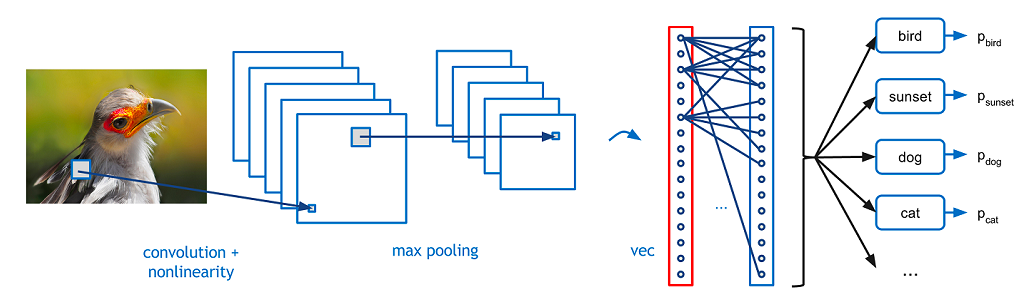
\includegraphics[width=0.95\textwidth]{Tesi/images/image_classification}
\caption{Image Classification using a \ac{CNN}.}
\label{fig:first_figure}
\end{figure}

\newpage

One of the most interesting peculiarity of \acp{CNN} applied to the task of image classification is their ability to explain which part of the picture they are looking at while assigning the class. This can be done by producing a \ac{CAM}, a 2D grid of scores computed for every location of the input image, indicating how important is each location with respect to a given class. Figure~\ref{fig:second_figure} shows an example of \ac{CAM}s produced while assigning the labels "cat" and "dog" to the image given as input. As we can see the network is looking at the correct part of the image, paying attention at the top area to classify the dog and at the bottom one to classify the cat. 

\begin{figure}[htbp!]
\centering
\includegraphics[width=0.85\textwidth,height=0.2\textheight]{Tesi/images/CAM}
\caption{Example of Class Activation Map \cite{cam_paper}.}
\label{fig:second_figure}
\end{figure}


\subsection{Deep Learning in Chest X-Ray Diagnosis}
\label{subsec:convolutional_neural_networks}
During the last years the problem of \ac{CXR} diagnosis has been tackled multiple times using different approaches. One of the major drawbacks of \ac{DL} is that it requires a massive amount of data in order to achieve good results. The first public dataset containing a significant amount of labeled radiography is "ChestX-ray8", that has been release in 2017 by the National Institute of Health \cite{Wang_2017}. It is composed by 108,948 frontal-view X-Ray images coming from 32,717 unique patients. Each radiography is associated with 8 different labels (subsequently increased to 14), each one referring to a particular disease. Among the large amount of work that has been done by the scientific community using this dataset, it worth mentioning that of Rajpurkar et al. \cite{rajpurkar2017chexnet}, able to achieve performance statistically significantly higher than radiologist. In 2019 two new dataset has been released: Chexpert~\cite{irvin2019chexpert}, composed by 224,316 chest radiographs of 65,240 patients, and MIMIC-CXR-JPG~\cite{johnson2019mimiccxrjpg}, made of 377,110 images. \ac{CXR}s from the two dataset are provided with the same 14 labels, that have been extracted from radiology report using \ac{NLP}. 
\newpage
\section{Neural Networks}
\label{sec:Neural Network}
\acp{FCNN} are a computing system able to catch the relationship binding an input to an output. They are based on a Supervised Learning paradigm: in order to learn the function mapping an input to its corresponding output, the network must be trained using a lot of examples composed by both the input and the desired output. 
\vspace{5mm}

A \ac{FCNN} is made of a series of hidden layers, each one composed by a given number of elementary units, called artificial neurons, that are fully connected to the ones belonging to the previous layer. When the network receives an input, it pass through all the network and gets transformed by the artificial neurons, until it reaches the last layer, where an output is carried out (Figure \ref{fig:third_figure}).
\begin{figure}[htbp!]
\centering
\includegraphics[scale=0.45]{Tesi/images/FCNN}
\caption{Fully Connected Neural Network}
\label{fig:third_figure}
\end{figure}

\vspace{5mm}
This model, however, is not suitable for image processing. Indeed, if we consider, for example, an image with shape $32 \times 32 \times 3$ pixels, a single neuron in the first hidden layer of a \ac{FCNN} would have a number of connections equal to 32*32*3 = 3072. Although it seems to be a reasonable amount of weights, this approach does not scale well when we are dealing with larger images. As we will see in next chapters, our images will have a size of $224 \times 224 \times 3$, using \ac{FCNN} would lead a single neuron to have 150,528 connections. Such a number of parameter is intractable and would lead to overfitting.

\subsection{Convolutional Neural Network}
\label{sec:convolutional_neural_network}
Convolutional Neural Networks are a particular type of Neural Networks that have been extensively used over the past years, able to overcome the limits of \ac{FCNN} discussed in section \ref{sec:Neural Network}. \acp{CNN} have been successfully used for the first time by Yann Lecun for the task of recognizing handwritten digits \cite{lecun}.
The most important building block introduced with \acp{CNN} is the convolutional layer, designed to take advantage of the multi-dimensional structure of the input. Neurons in the first convolutional layer are not connected to every single pixel of the input image, but only to a small part of it, the so called receptive field. \acp{CNN} have a hierarchical structure: in the first layers the network extracts simple patterns, such as edges and curves that, in the following layers, are assembled to generate higher level features (Figure \ref{fig:fourth_figure}).
\begin{figure}[htbp!]
\centering
\includegraphics[width=0.90\textwidth]{Tesi/images/Feature}
\caption{Feature hierarchy in a \ac{CNN}}
\label{fig:fourth_figure}
\end{figure}

Feature extraction is accomplished by the so called kernels (also known as filter). Figure \ref{fig:fifth_figure} shows an example of two kernels applied to an image: in the top left picture a vertical filter has been used, thus all the vertical lines in the original image gets enhanced, while the rest gets blurred. The top-right image, instead, shows what happen when an horizontal filter is applied. Of course kernels do not have to be defined manually, during the training phase the convolutional layers will automatically learn the most useful for the given task and the subsequent layers will learn to combine them into more complex pattern.
\vspace{5mm}
\begin{figure}[htbp!]
\centering
\includegraphics[scale=0.8]{Tesi/images/FeatureMap}
\caption{Example of filters applied to an image \cite{mlbook}}
\label{fig:fifth_figure}
\end{figure}

\vspace{5mm} %5mm vertical space

The mathematical operation that allows the network to extract the features from the input image is called convolution, that consist in sliding a kernel (that is basically a small matrix of number), across the whole dimensions of the input and compute the dot product between the entries of the filter and the input at any position. Convolution between image $I$ and kernel $w$ of size $k \times k$ can be computed as:
\begin{equation} \label{eq:first_equation}
\begin{gathered}
(I\ast w)\left [ r,c \right ]  = \sum_{x=-k}^{k}  \sum_{y=-k}^{k} w(x,y)I(r-x, c-y)
\end{gathered}
\end{equation}

\noindent An example of convolution is shown in Figure \ref{fig:sixth_figure}, in which the value of the destination pixel has been computed as: 
\begin{equation} \label{eq:second_equation}
\begin{gathered}
(4 \cdot  0) + (0 \cdot  0) + (0 \cdot  0) + (0 \cdot  0) + (0 \cdot  1) + (0 \cdot  1) + (0 \cdot  0) + (0 \cdot  1) + (-4 \cdot  2) = -8
\end{gathered}
\end{equation}

\begin{figure}[htbp!]
\centering
\includegraphics[scale=0.7]{Tesi/images/convolution}
\caption{Example of convolution operation between an image and a kernel}
\label{fig:sixth_figure}
\end{figure}

\newpage

\vspace{5mm} %5mm vertical space
\noindent Another widely used layer in \acp{CNN} is the Pooling Layer. Its function is to progressively decrease the spatial size of the representation in order to reduce the computational load, the memory usage and the number of parameter (preventing thereby the risk of overfitting). A pooling layer has no weights, what it does is to aggregate the input using an aggregation function, such as mean or max (Figure \ref{fig:seventh_figure}). A max pooling layer, moreover, introduces some level of invariance to small translations, a feature that could be useful for the task of image classification.


\begin{figure}[htbp!]
\centering
\includegraphics[width=0.95\textwidth]{Tesi/images/pooling}
\caption{Example of Max Pooling}
\label{fig:seventh_figure}
\end{figure}

\subsection{Class Activation Map}
\label{sec:cam}
In 2016 Zhou et al. \cite{zhou2015cnnlocalization} shown that a \ac{CNN} is able to identify exactly which region of an image is used for discrimination. The novelty with respect to previous works is that the network is only trained for solving the  classification task, thus no bounding box annotation is provided as input to the network. 
The remarkable localization ability of \ac{CNN} is lost when the fully connected layer is used for classification. Thanks to the work of Lin et al. \cite{gap}, this problem can be overcome by means of a \ac{GAP} layer, initially introduced to minimize the number of parameters, avoiding the usage of fully connected layer while maintaining high classification performance. 
Similarly to Pooling Layers, a \ac{GAP} layer aims at reducing the spatial dimension of the input tensor. However \ac{GAP} makes a more extreme type of dimensionality reduction, transforming a three dimensional input of size $h \times w \times d$ into a tensor with shape $1 \times 1 \times d$ (Figure \ref{fig:eigth_figure}).

\begin{figure}[htbp!]
\centering
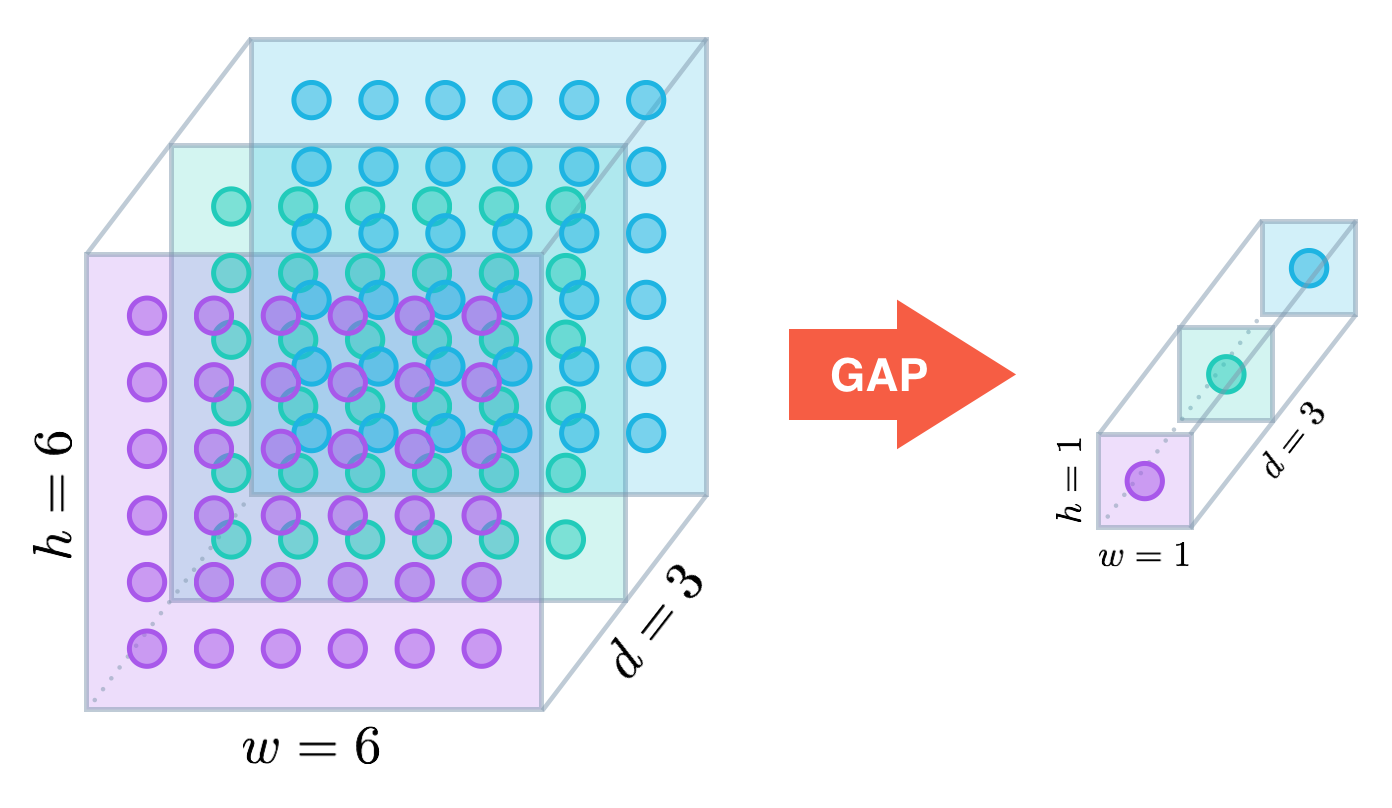
\includegraphics[scale=0.5]{Tesi/images/GAP}
\caption{Example of Globale Average Pooling \cite{gap_image}.}
\label{fig:eigth_figure}
\end{figure}

\noindent In order to generate the \ac{CAM}, we will make a weighted sum of the feature maps at the last convolutional layer. If we indicate with $f_{k}(x,y)$ the activation of unit k at spatial location $(x,y)$ then the result of performing Global Average Pooling is given by:

  \begin{equation}
  \label{eq:third_equation}
  \begin{gathered}
  F_{k} = \sum_{x,y} f_{k}(x,y)
  \end{gathered}  
  \end{equation}
  
\vspace{3mm}

\noindent Thus the input to the softmax for a given class will be:
 \begin{equation}
  \label{eq:fourth_equation}
  \begin{gathered}
  S_{c} = \sum_{k} w_{k}^{c} F_{k} = \sum_{x,y} \sum_{k} w_{k}^{c} f_{k}(x,y)
  \end{gathered}  
  \end{equation}
  
\vspace{3mm}

\noindent Essentially $w_{k}^{c}$ represent the importance of $F_{k}$ for class $c$. Once $S_{c}$ has been calculated, the probability for a class $c$ can be computed using the softmax function: 
\begin{equation}
\label{eq:fifth_equation}
\begin{gathered}
P_{c} = \frac{exp(S_{c})}{\sum_{c} exp(S_{c})}
\end{gathered}  
\end{equation}
\vspace{3mm}

\noindent While the Class Activation Map for class $c$, instead, can be computed as : 

  \begin{equation}
\label{eq:sixth_equation}
\begin{gathered}
M_{c}(x,y) = \sum _{k} w_{k}^{c} f_{k}(x,y)
\end{gathered}  
\end{equation}
  
\noindent So in order to extract the most important part of the image for a given class, we project back the weights of the output layer on the convolutional feature maps obtained from the last Convolution Layer. Image \ref{fig:ninth_figure}, taken from the work of Zhou et al. \cite{cam_paper}, shows how the \ac{CAM} is computed by making a weighted sum of the last convolutional layer's features.

\begin{figure}[htbp!]
\centering
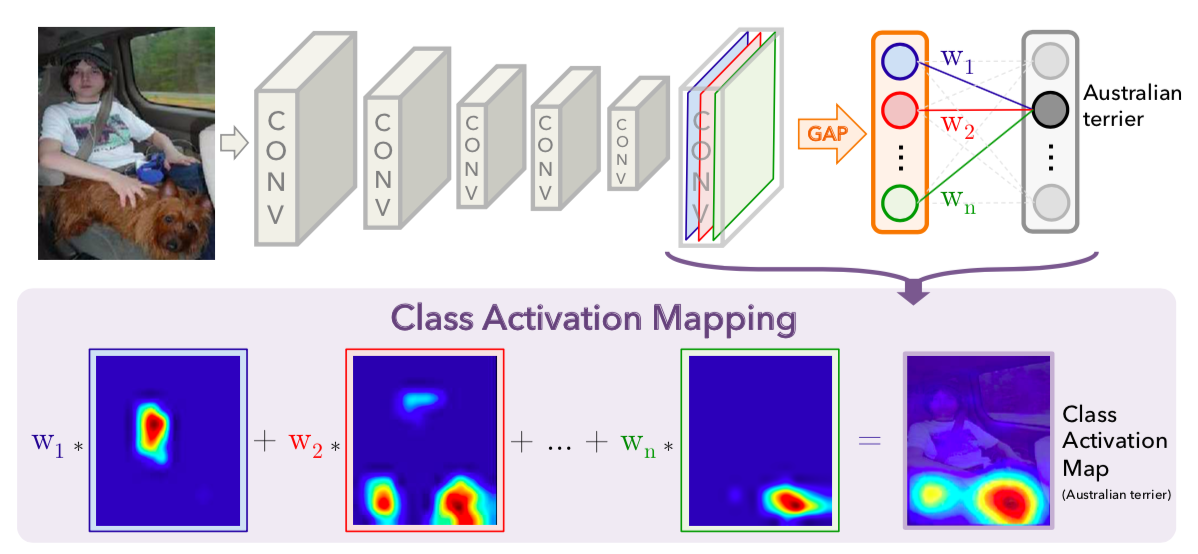
\includegraphics[scale=0.35]{Tesi/images/Class Activation Map}
\caption{Class Activation Map generation.}
\label{fig:ninth_figure}
\end{figure}

\subsection{Embedding}
\label{sec:embedding}
In the context of \ac{ANN} a very useful techniques is Embedding. When dealing with images, we generally work with a massive amount of data. A simple colored image with resolution of $224 \times 224$ pixels is converted into a tensor having $224 \times 224 \times 3 = 150.528$ entries. Although \acp{CNN} are able to deal with such a large amount of data, the vast majority of algorithms can't process it in a reasonable amount of time.
In order to overcome this issue we can rely on Embedding, a set of techniques used to reduce the input dimension. An embedding is a learned low dimensional vector representing the input. Once an embedding has been extracted, it somehow contains the same relevant information of the input but in a smaller and more manageable representation, suitable for being used by other kind of algorithms. 

\vspace{5mm}

\acp{CNN} can be used to extract the low dimensional feature vector. In the hidden layers, in fact, the network learns a representation of the input that is subsequently used for classification. If we cut the network at one of the hidden layer, thus, we can extract a low dimension vector representing the the input (Figure \ref{fig:tenth_figure}).


\begin{figure}[htbp!]
\centering
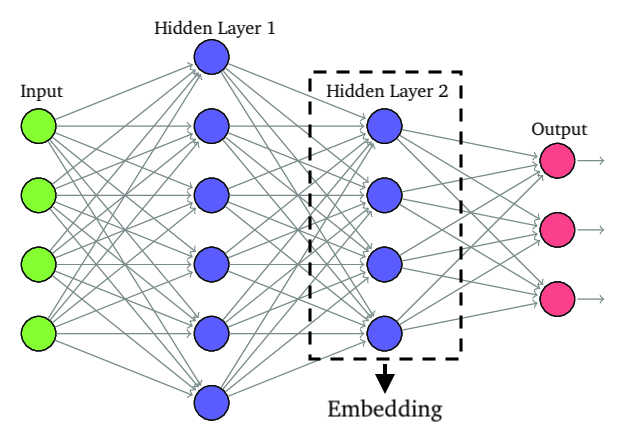
\includegraphics[scale=0.5]{Tesi/images/Embedding}
\caption{Embedding extraction from an \ac{ANN}}
\label{fig:tenth_figure}
\end{figure}


\section{Ensemble Learning}
\label{sec:ensemble}
In social science there is a theory, called "The Wisdom of Crowd", stating that the aggregate decision made by a group of people will often be better than those of it's individual members \cite{crowd}. A similar idea is exploited by Ensemble Learning, a technique that allows to improve machine learning results by combining several models. Figure \ref{fig:eleventh_figure} shows a typical workflow exploiting ensemble: several classifiers are trained and then combined in order to carry out a single prediction that takes care of the opinion coming from all the base classifiers. 
\begin{figure}[htbp!]
\centering
\includegraphics[scale=0.35]{Tesi/images/Ensemble.pdf}
\caption{Ensemble Learning}
\label{fig:eleventh_figure}
\end{figure}
The keypoint here is to find the best way to combine all the predictions. There are  different approaches, such as:
\begin{itemize}
  \item \textbf{Ensemble Averaging}: the predictions that are carried out from the single experts are merged together using either a mere average or a weighted sum. Doing this helps reducing the variance of the output.
  For example, if we indicate as $y_{i}$ the output of each base classifier, then the ensemble of the $n$ experts can be computed as:
  \begin{equation}
  \label{eq:seventh_equation}
  \begin{gathered}
  \bar{y}(\mathbf{x},\alpha) = \sum_{i=1}^{n} \alpha_i y_{i}(\mathbf{x})
  \end{gathered}  
  \end{equation}
  \item \textbf{Bootstrap Aggregating}: also known as Bagging \cite{bagging}, this technique aims at reducing the variance by averaging the output of multiple models built on different training set. More specifically, given a dataset $D$, each model if fitted using a dataset $D_{i}$ build by sampling uniformly and with replacement from $D$.
  
  \item \textbf{Boosting}: this aggregation approach aims at producing a strong predictor by incrementally building the weak classifiers. It's peculiarity is that each model instance is trained paying more attention to the samples that were misclassified by the previous predictor.
  
  
  \item \textbf{Stacking}: this approach combines multiple classification or regression models using a meta-classifier or a meta-regressor. Specifically, a training set is used to train the base classifiers, then the predictions that are carried from the classifiers are used as feature to train the meta-learner. The pseudocode for the general stacking algorithm is shown in figure \ref{fig:twelfth_figure}
  \begin{figure}[htbp!]
\centering
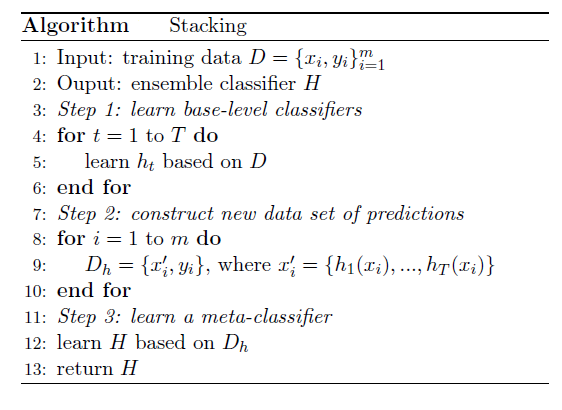
\includegraphics[scale=0.55]{Tesi/images/stacking_pseudocode.png}
\caption{Stacking Pseudocode}
\label{fig:twelfth_figure}
\end{figure}
  
    \end{itemize}


\section{Random Forest}
\label{sec:random_forest}
Random Forests are an ensemble algorithm proposed by T.K. Ho in 1995 \cite{random_forest}. The idea behind \acp{RF} is to build a multitude of decision trees and combine their predictions.

\noindent Decision Trees are a supervised-learning method used bot for classification and regression tasks. The algorithm builds a tree-like structure in which:
\begin{itemize}
    \item An internal node is a test on an attribute.
    \item A branch represent an outcome of the test.
    \item A leaf represent a class label or a class label distribution.
\end{itemize}


\noindent Figure \ref{fig:thirteenth_figure} shows an example of Decision Tree used to predict survivals on Titanic. A new instance is assigned to a class by following a path starting from the root and ending in a leaf node, testing a different feature at each internal node.

\begin{figure}[htbp!]
\centering
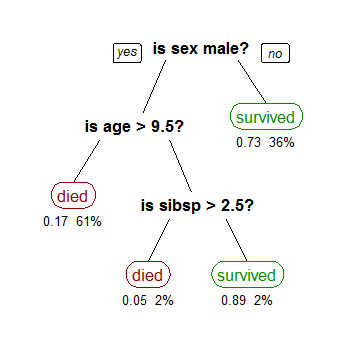
\includegraphics[scale=0.7]{Tesi/images/CART_tree_titanic_survivors.png}
\caption{Decision Tree showing survival of passenger on Titanic \cite{pict}}
\label{fig:thirteenth_figure}
\end{figure}
  
Decision Trees have many advantages: they are very fast in making predictions and, differently from \acp{ANN}, they are a white box model, in the sense that they are easy to interpret and visualize. Indeed it's possible to easily check which are the features that most contribute to carry out a particular prediction. However, they also have some drawback. They often create over-complex structure that are not able to generalize well, thus leading to overfitting. Another big issue is that they are unstable, in the sense that a small variation in the training data may generate a totally different model.
These issues can be overcome by resorting to Random Forest, that are basically an ensemble of Decision Trees based on Bagging, a technique seen in section \ref{sec:ensemble}.
The main steps to build a Random Forest are the following:
\begin{itemize}
    \item Build $k$ training set $D_{i}$ by sampling with replacement from $D$
    \item Learn tree $T_{i}$ from $D_{i}$ using only a random subset of the input variables.
    \item Save the tree as it is, without performing any pruning
\end{itemize}
Once the Random Forest has been created, the predictions computed by the trees are combined using:
\begin{itemize}
    \item Majority Voting (in the case of Classification)
    \item Average (in the case of Regression)
\end{itemize}

When the number of trees is sufficiently large, Random Forest can prevent overfitting. Moreover they are an easy to use tool, having only two important parameters to tune (number of trees and percentage of variables for split).
  \begin{figure}[htbp!]
\centering
\includegraphics[scale=0.35]{Tesi/images/rf.pdf}
\caption{Example of Random Forest for classification task}
\label{fig:fourteenth_figure}
\end{figure}


\section{Gradient Boosting}
\label{sec:gradient_boosting}
Gradient Boosting is a learning algorithm proposed in 1990 by Friedman \cite{gradient_boosting}. As the name suggests, it's a technique based on boosting. The idea of this algorithm can be summarized by the following steps:
\begin{enumerate}
    \item Learn a predictor.
    \item Compute the error residual.
    \item Learn to predict the residual
    \item Goto point 2
\end{enumerate}

\noindent So Gradient Boosting tries to repetitively leverage the patterns in the residuals to improve the successive predictions.
The predictors used as weak leaerner in gradient boosting are decision trees. Note that, however, gradient boosting is a greedy algorithm and, thus, it can overfit the dataset quickly. A solution to this problem is that of constraining the trees, being the shallow trees, generally, less prone to overfitting.


\section{Summary}
\label{sec:sec_chapter_sumary}
The goal of this chapter was to give an general overview of the main techniques that will be used in the following chapters. We've seen what Artificial Neural Networks are and how they can be used in order to deal with images, both for classify them and localize interesting areas. We've also seen how multiple approaches can be combined together to enhance the global performance, with a particular attention on Random Forest. In the next chapter we will introduce the dataset and we'll describe the pre-processing phase.
\chapter{Chest X-Rays Automated Diagnosis}
\label{cha:third_chapter}

The goal of this chapter is to formally present the problem and introduce the dataset that we will use to train, evaluate and test the models that will be presented in the following chapter. In particular we want to give a description about the content of the dataset, its structure and also the pre-processing steps that have be done. 

\section{Problem Formulation}
\label{sec:problem_formulation}
The focus of this work is to build a system able to make accurate diagnoses of 14 different diseases analyzing an input image containing a chest x-ray. Formally, we have a dataset $D = \{(\mathbf{x}^{(\mathit{i})},\mathbf{y}^{(\mathit{i})}) ;\mathit{i}:1,...,N \}$ containing $N$ \acp{CXR}, where each image $\mathbf{x}^{(\mathit{i})}$ is associated with a set of label $\mathbf{y}^{(\mathit{i})} \in \{0,1\}^{14}$, where a value of 0 means that the corresponding disease is not present on the given input, while a value of 1, instead, means that it's present. We want our system to be able to predict, given a new instance $\mathbf{x}^{(\mathit{i})}$, the corresponding output  $\mathbf{y}^{(\mathit{i})}$. To be more specific, our system will carry out a value corresponding to the probability, for each pathology, to be present or not on a given \ac{CXR}. It is worth noting that this is not a multiclass classification problem, in which there is the assumption that a sample can be assigned to one and only one class, but it's a multilabel classification problem, in which a sample can be assigned to an arbitrary number of classes.

\vspace{3mm}
We also want our model to be able to produce a map highlighting the area of the image interested by the pathology and use it to automatically extract a bounding box around the disease region.

\section{Data Source}
\label{sec:data_source}
In our work we've decided to use CheXpert (\textbf{Che}st e\textbf{Xpert}), a large dataset released in 2019 by Stanford University for \ac{CXR} examination \cite{irvin2019chexpert}. 

\subsection{Content}
\label{sec:dataset_content}
The dataset is composed by 223,316 chest x-rays of 65,240 patients, collected by Stanford Hospital from October 2002 to July 2017.
The dataset is offered at two quality levels: the high quality one has a size of 439GB and the images are stored as 16-bit PNG, while the small version has a size of 11GB and stores the chest x-rays using a 8-bit PNG format. In this work, due to computational reasons, we have decided to use the small version.

\noindent Each image is annotated with 14 labels, that have been extracted from text radiology report using an automatic rule-based labeler. The labelling process can be divided in three different phases:
\begin{itemize}
    \item Mention Extraction: the \textit{Impression} section of the radiology report, which summarizes the key finding in the radiology study, is analyzed and a list of mentions is extracted. The extracted mentions are those that match a large list of phrases that has been manually created by multiple expert radiologist.
    \item Mention Classification: this phase aims at assigning each mention to a label among:
    \begin{itemize}
        \item Positive: the disease is confidently present
        \item Negative: the disease is confidently absent
        \item Uncertain: this value captures both the uncertainty in the radiologist diagnosis as well as the inherent ambiguity of the report.
    \end{itemize}
    \item Mention Aggregation: the last phase aggregates the classification of all the mentions in order to generate a label for all the 14 observations. Each label is assigned a positive (1), negative (0) or uncertain (\textit{u}) value if it has been explicitly mentioned in the report, while the (\textit{blank}) value is assigned to the unmentioned observations. 
\end{itemize}

\noindent The labeller has been tested by the Stanford Team against human labelled cases, showing that it is able to achieve very high perfomance.

\newpage
\noindent The labels have a hierarchical structure, that has been provided along with the dataset and can be seen in Figure \ref{fig:figure_3_1}. As we can see, for example, there is a dependency between Lung Opacity and Edema, meaning that an X-Ray presenting Edema must also contain a Lung Opacity (but the contrary must not necessarily be true). 

\begin{figure}[htbp!]
\centering
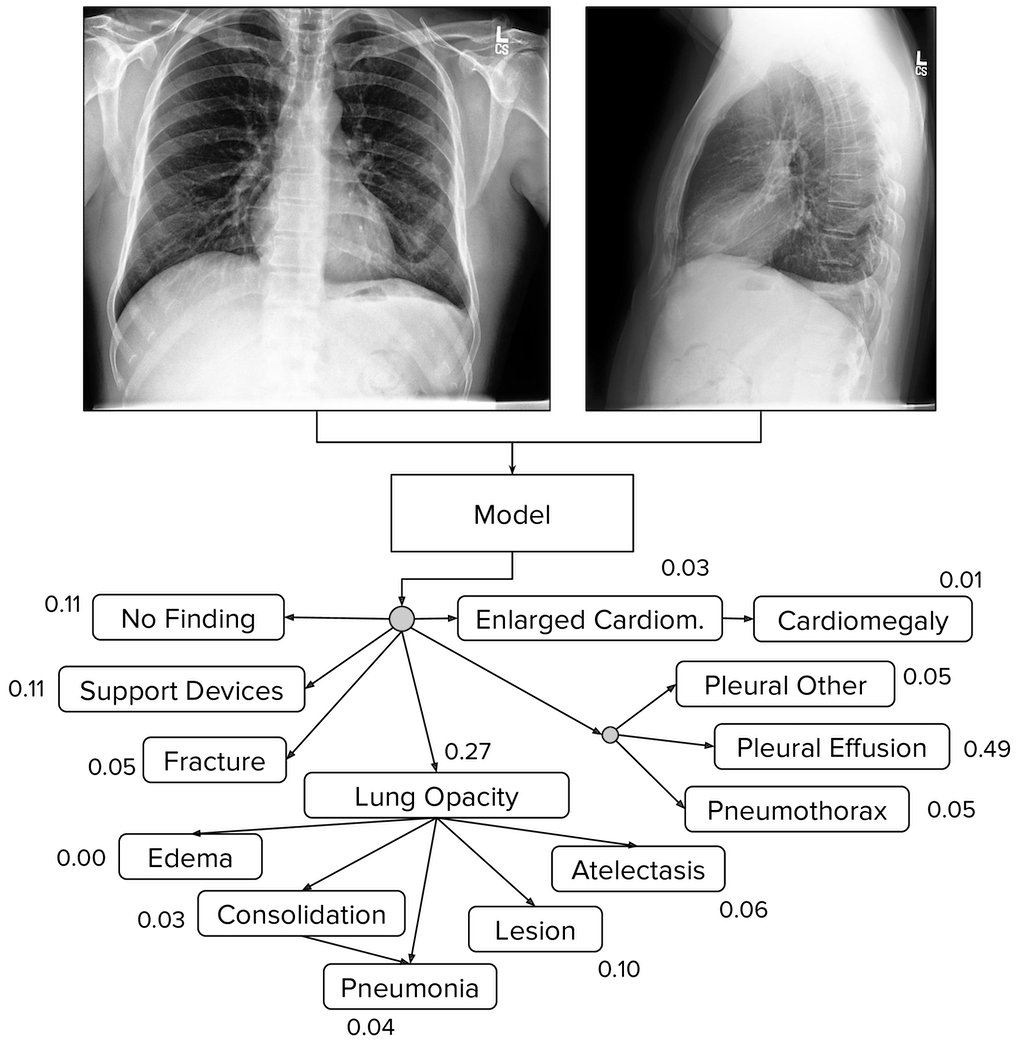
\includegraphics[scale=0.26]{Tesi/images/label_hierarchy}
\caption{Pathologies hierarchy}
\label{fig:figure_3_1}
\end{figure}

\noindent This additional information can be exploited in order to enhance the quality of the predictions.

\noindent Table \ref{table:table_1} gives a brief description of all the medical conditions that have been considered in the dataset. 

\newpage

\begin{table}[h!]

\centering

\begin{tabularx}{\textwidth}{|l|X|}
\hline
\textbf{Pathology Name}    & \textbf{Description}                                                                                 \\ 
\hline
No Finding                 & No pathology is assigned to a positive or uncertain label                                            \\ 
\hline
Enlarged Cardiomediastinum & Abnormal enlargement of the cardiomediastinal~silhouette                                             \\ 
\hline
Cardiomegaly               & Condition where the heart is enlarged.                                                                \\ 
\hline
Lung Lesion                & Damaged portion of a lung.                                                                           \\ 
\hline
Lung Opacity               & Area that attenuates x-ray beams, making the lung appearing more opaque than the surrounding region.  \\ 
\hline
Edema                      & Fluid accumulation in the tissue and air spaces of the lung.                                                                                                 \\ 
\hline
Consolidation              & Region of normally compressible lung tissue that has filled with liquid instead of air. The condition is marked by induration.                                                                                                    \\ 
\hline
Pneumonia                  & Pneumonia is an infection that inflames the air sacs in one or both lungs.                                                                                                      \\ 
\hline
Atelectasis                & Collapse or closure of a lung resulting in reduced or absent gas exchange.                                                                                                     \\ 
\hline
Pneumothorax               & Condition in which air accumulates in the pleural sac, causing it to expand and compress the underlying lung.                                                                                                     \\ 
\hline
Pleural Effusion           & Excess of fluid that accumulates in the pleural cavity.                                                                                                     \\ 
\hline
Pleural Other              & Other pleural disease                                                                                                      \\ 
\hline
Fracture                   & Partial or complete break in the continuity of a bone.                                                                                                      \\ 
\hline
Support Device             & Medical device aims at supporting or sustaining patient's life.                                                                                                      \\
\hline
\end{tabularx}
\caption{Definition of all the diseases considered in the dataset}
\label{table:table_1}
\end{table}



\subsection{Structure}
\label{sec:dataset_structure}
As mentioned in the previous section, the dataset contains 224,316 chest X-Rays extracted from 65,240 different patients. The details about the distribution of the different labels are reported in Table \ref{table:table_2}.


\begin{table}[h!]
\centering
\begin{tabular}{|l|l|l|l|} 
\hline
\textbf{Pathology}         &  \hfill \textbf{Positive (\%)}& \hfill \textbf{Uncertain (\%)}  & \hfill \textbf{Negative (\%)}   \\ 
\hline
No Finding        &    \hfill16627 (8.86)&      \hfill   0 (0.0)  & \hfill171014 (91.14)    \\\hline
Enlarged Cardiom. &    \hfill 9020 (4.81)&   \hfill 10148 (5.41)  & \hfill168473 (89.78)    \\\hline
Cardiomegaly      &  \hfill 23002 (12.26)&    \hfill 6597 (3.52)  & \hfill158042 (84.23)    \\\hline
Lung Lesion       &   \hfill  6856 (3.65)&   \hfill  1071 (0.57)  & \hfill179714 (95.78)    \\\hline
Lung Opacity      &  \hfill 92669 (49.39)&   \hfill  4341 (2.31)  & \hfill90631 (48.3)  \\\hline
Edema             &  \hfill 48905 (26.06)&   \hfill 11571 (6.17)  & \hfill127165 (67.77)    \\\hline
Consolidation     &  \hfill  12730 (6.78)&   \hfill23976 (12.78)  & \hfill150935 (80.44)    \\\hline
Pneumonia         &  \hfill   4576 (2.44)&   \hfill 15658 (8.34)  & \hfill167407 (89.22)    \\\hline
Atelectasis       & \hfill  29333 (15.63)&  \hfill 29377 (15.66)  & \hfill128931 (68.71)    \\\hline
Pneumothorax      & \hfill   17313 (9.23)&   \hfill  2663 (1.42)  & \hfill167665 (89.35)    \\\hline
Pleural Effusion  &  \hfill 75696 (40.34)&   \hfill  9419 (5.02)  & \hfill102526 (54.64)    \\\hline
Pleural Other     &  \hfill    2441 (1.3)&   \hfill  1771 (0.94)  & \hfill183429 (97.76)    \\\hline
Fracture          &  \hfill   7270 (3.87)&   \hfill   484 (0.26)  & \hfill179887 (95.87)    \\\hline
Support Device    &  \hfill 105831 (56.4)&   \hfill   898 (0.48)  &  \hfill80912 (43.12)   \\
\hline
\end{tabular}
\caption{Number of Positive, Uncertain and Negative labels for each disease}
\label{table:table_2}
\end{table}

The Stanford Team also provided a set of manually labeled images that can be used to assess the performance of the predictions. We additionally cut out a subset of data that will be used to tune the models' hyperparameters.
The dataset, moreover, contains two type of \acp{CXR}, the frontal-view and the lateral-view. Generally the latest one is performed as an adjunct to a frontal chest radiograph in cases where there is a diagnostic uncertainty. For this reason, the number of frontal images is much higher. The following table reports the numerical details about the dataset composition.

\vspace{5mm}

\begin{table}[h!]
\centering
\begin{tabular}{|l|l|l|} 
\hline
\textbf{Dataset}         &   \hfill \textbf{Frontal (\%)} &   \hfill \textbf{Lateral (\%)} \\
\hline
Training &    \hfill 189116 (84.56)   & \hfill 32387 (14.48) \\\hline
Validation &    \hfill 1911 (0.85)   & \hfill 0 (0.00)\\\hline
Test &    \hfill 202 (0.09) & \hfill 32 (0.01) \\

\hline
\end{tabular}
\caption{Dataset structure}
\label{table:table_3}
\end{table}


\section{Preprocessing}
\label{sec:preprocessing}
In this section we describe the preprocessing steps that have been done on the data before submitting them to the learning algorithms.

\vspace{5mm}

\noindent\textbf{Labels}

\vspace{5mm}

\noindent The author of the dataset provided, together with the images, two \textbf{.csv} files (one for the training set and one for the test set) mapping each \ac{CXR} with its own set of labels. Moreover, each image has additional information about the gender and the age of the patient that, however, in this work have not been considered. We also decided to focus our attention on the Frontal Chest X-Rays only, discarding the Lateral ones, that were available only for a relatively small amount of patients.

\noindent These are the steps we have done in order to clean the \textbf{.csv} files: 
\begin{itemize}
    \item The columns \textbf{"Sex"}, \textbf{"Age"}, \textbf{"Frontal/Lateral"}, \textbf{"AP/PA"} have been removed.
    \item The \textit{blank} values (i.e the unmentioned labels) have been assigned a value of 0.
    \item The uncertain labels, indicated with value -1, have been assigned a value that depends on the policy that have been used to deal with the uncertainties (we will give a more detailed explanation in section \ref{sec:uncertainty}).
\end{itemize}

\noindent The final \textbf{.csv} files were composed by a column containing the image reference and 14 additional columns, one for each disease, filled with a value indicating whether a particular pathology is present, not present or uncertain.


\vspace{5mm}

\noindent\textbf{Images}

\vspace{5mm}

\noindent Most of the images were affected by irrelevant noise such as text or irregular borders. Since these areas might affect the learning performance, we tried to solve the problem by removing them. So the \ac{CXR} images were first resized to $256 \times 256$ pixels and then a template matching algorithm has been applied in order to find a region of the image with size $224 \times 224$ containing a chest template. In many cases this approach successfully removed the irrelevant areas, as we can see in Figure \ref{fig:figure_3_2}. Moreover, the images have been converted to RGB in order to match the required input shape of the models and pixel values have been scaled in a range between 0 and 1. Finally, since the model we have used have been pre-trained on ImageNet \cite{imagenet}, we have normalized all the images with respect to mean and standard deviation of that dataset.

\vspace{5mm}


\begin{figure}[h!]
\centering
\begin{minipage}{.4\textwidth}
  \centering
  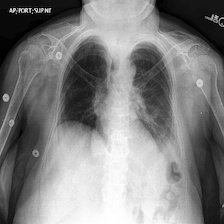
\includegraphics[width=5cm]{Tesi/images/img1}
  \caption*{Before}
\end{minipage}%
\begin{minipage}{.4\textwidth}
  \centering
  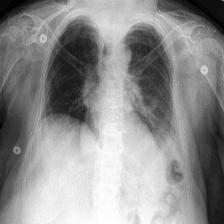
\includegraphics[width=5cm]{Tesi/images/img2}
  \caption*{After}

\end{minipage}
\caption{Comparison of \ac{CXR} before and after preprocessing}%
\label{fig:figure_3_2}
\end{figure}

\newpage
\noindent\textbf{Data Format}

\vspace{5mm}

\noindent When dealing with very large amount of data, using the proper data format could have a significant impact on the performance of the input pipeline and, consequently, on the training time of the model. In our work we have decided to use the TFRecord data format, that is Tensorflow’s own binary storage format.
TFRecord is extremely useful when dealing with large dataset that does not fit in RAM, because it allows to efficiently load and preprocess only the data that are required at the time. 
\noindent Each entry of our TFRecord file is composed by two elements: 
\begin{itemize}
    \item Image: serialized version of a \ac{CXR}
    \item Labels: vector of 14 elements, each one associated to a particular pathology.
\end{itemize}

\section{Related Works}
\label{sec:related_work}
Since it's introduction, there have been many works involving CheXpert. The first one has been released together with the dataset, in which the Stanford team developed a system able to classify and localize the different diseases exploiting a \ac{CNN}. Moreover, they explored different approaches to deal with the uncertain labels and, finally, compared their results with that of 3 radiologist, exceeding their score in most of the pathologies. 

\noindent The Stanford Machine Learning Group also set up a competition, called CheXpert \cite{chexpert_competition}, that allows people from all over the world to submit the result of their projects involving CheXpert. Among the different works, it worth mentioning that of Pham et al. \cite{pham2019interpreting}, that reached the first position on the competition. The key point of their work is the investigation of novel approaches to deal with the uncertain labels, the use of Ensemble, and the exploitation of the dependency among the diseases to improve the quality of the prediction.

\section{Summary}
\label{sec:summary_chapter_three}
In this chapter we have introduced the dataset that we will use in our work, presenting its composition and its structure. We have also also talked about the preprocessing steps that we have done before submitting the data to the training algorithms and, finally, we mentioned the related works that have been done involving the same dataset. In the next chapter we will dive into the core of this work, presenting a formal definition of the problem and the solution we have developed to solve it. 
\chapter{System Design}
\label{cha:fourth_chapter}

In this chapter we will present the approaches we have developed to solve the problem of classifying and localize the different diseases on a given Chest X-Ray. We will first talk about the approach we used to deal with uncertain labels, then we will present the models that we've developed to identify the different pathologies and we'll show the techniques that have been used to aggregate them. Finally, we will talk about the approach we've used to identify the region of the CXR affected by the disease. 


\section{Uncertain Labels}
\label{sec:uncertainty}
As already introduced in Chapter \ref{cha:third_chapter}, the dataset contains a significant number of diseases that have been labelled as uncertain. The uncertainty could reflect both an unreliable diagnosis or an ambiguity in the report. In their work, Irvin et al. \cite{irvin2019chexpert}, proposed different policies to deal with them:
\begin{itemize}
    \item U-Ignore: this is the simplest approach, that consists in ignoring all the uncertain labels during the training. This method, however, could produce biased models and also reduce the effective size of the dataset if the number of uncertain labels is significant.
    \item U-Zeros: this approach consists in assigning a 0 label to the uncertain one, thus considering the associated disease as not present.
    \item U-Ones: this is similar to the previous method but, instead of considering the uncertain labels as negative, they are considered as positive, thus they are assigned a label equal to 1.
    \item U-SelfTraining: with this method, the uncertain labels are first considered as unlabeled examples. Then a model is  trained using the U-Ignore policy and, finally, it is used to make predictions in order to re-label each uncertain label.
    \item U-MultiClass: the last policy treats the \textit{u} label as its own class. Thus, for each pathology, three different probabilities $\{p_{0} , p_{1},p_{u}\}$ are carried out, each one representing the probability of belonging to, respectively, class $0$, $1$ or $u$.
\end{itemize}

Focusing our attention on U-Zeros and U-Ones policy, Pham et al. \cite{pham2019interpreting}, in their work, put the evidence on a problem related to these two approaches: mapping all the uncertainty to either 0 or 1 will certainly result in a lot of wrong labels and, consequently, the model would be misguided during training. Thus, they used a technique called \ac{LSR}, introduced by Szegedy et al. \cite{lsr}, that allows to exploit the large amount of uncertain labels but preventing the model from becoming over confident about the prediction of examples that could contain mislabeled data.
Thus, the U-Ones policy has been modified by mapping each uncertain label to a random number close to 1. Formally, we have:
\begin{equation}
\scalebox{1.2}{
$
\bar{y}_{k}^{(i)} = \left\{\begin{matrix}
x, & \hfill \textup{if} \; y_{k}^{(i)}  = u\\ 
y_{k}^{(i)}, &\hfill  \textup{otherwise}
\end{matrix}\right.
$
}
    \label{eq:equation_4.1}
\end{equation}

\noindent where $x \sim U(a_{1},b_{1})$ is a randomly distributed number between $a_{1}$ and $b_{1}$. Similarly, the U-Zeros policy can be modified, mapping the uncertain labels to a number $x \sim U(a_{1},b_{1})$ close to 0.

\section{Convolutional Neural Network}
\label{sec:cnn}
In this section we talk about the first approach we've used, involving Artificial Neural Network. We start by describing the simplest model we've used and gradually we'll show how we have improved it.

\subsection{Single CNN And Training Procedure}
\label{sec:single_cnn}
The first approach we have investigated is the one involving a Convolutional Neural Network trained with U-Ones policy and \ac{LSR} (presented in the previous section). The uncertain labels, thus, have been mapped to a random number uniformly sampled between the interval $[0.55,0.85]$.

\vspace{3mm}
\subsubsection{Network Architecture}

\noindent Instead of training a Neural Network from scratch, we have decided to rely on Transfer Learning, using a Neural Network previously trained on a different dataset and retraining it in order to adapt to our new task. The architecture we used is the same already employed by Irvin et al. in their previous works \cite{irvin2019chexpert} \cite{rajpurkar2017chexnet}, called DenseNet121 and introduced for the first time in 2016 by Huang et al. \cite{densenet}. The peculiarity of this architecture is the use of dense connections that prevent the problem of vanishing information as the depth of the network increases. This problem is addressed by connecting each layer directly to each other in order to ensure the maximum information flow between them. Thus a layer receives the input from all the preceding layers and passes its own output to all the subsequent ones, as we can see in the example in Figure \ref{fig:figure_4.1} 

\begin{figure}[htbp!]
\centering
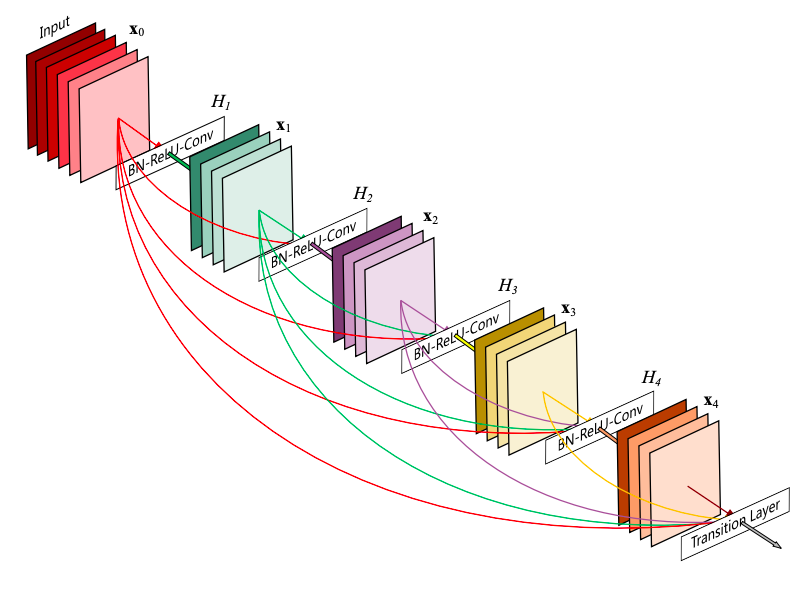
\includegraphics[scale=0.45]{Tesi/images/densenet}
\caption{Densely Connected Neural Network}
\label{fig:figure_4.1}
\end{figure}

The weights of the network have been initialized with that of the same network trained on the ImageNet dataset. The Fully Connected layer has been removed and substituted by a Global Average Pooling followed by a new \ac{FC} layer (note that the \ac{GAP} is essential for the production of a Class Activation Map).
The last layer produces a 14-dimensional output, after which we have applied an elementwise sigmoid function. If we call $z_{k}$ the output corresponding to the k-th label, the result of applying a sigmoid is: 
\vspace{3mm}

\begin{equation}
    y_{k} = \frac{1}{1+ exp(-z_{k})} , k = 1 \dots 14
    \label{eq:eq_4.2}
\end{equation}
\vspace{3mm}

\noindent The sigmoid function allows to squeeze $z_{k}$ in a range between $[0,1]$, thus we can give to $y_{k}$ a probabilistic interpretation.
\noindent Figure \ref{fig:figure_4.2} summarizes the overall network architecture:


\begin{figure}[htbp!]
\centering

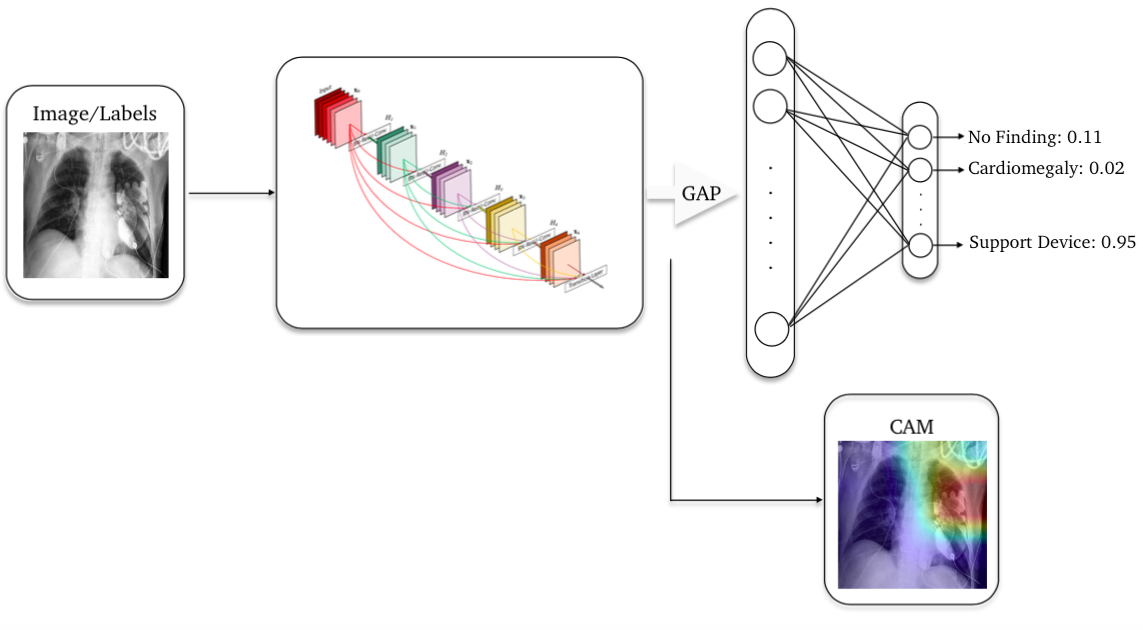
\includegraphics[scale=0.37]{Tesi/images/Architecture}
\caption{Network Architecture}
\label{fig:figure_4.2}
\end{figure}



\vspace{5mm}

\subsubsection{Training}

\noindent The network has been trained using Adam optimization algorithm \cite{adam} with default parameters $\beta_{1} = 0.9$ and  $\beta_{2} = 0.999$. The learning rate was initially set to $1e-4$ and then it has been gradually reduced by a factor of 10 at each epoch, allowing large weights changes at the beginning of the learning process and small changes towards the end. The number of epochs has been set to 10, but we also allowed the algorithm to early stop in case the optimization process show no more improvement on the validation set during the last 4 epochs. The objective function minimized by the optimizer is the binary cross entropy loss between the ground-truth labels and the predicted ones, who's formulation is the the following: 
\vspace{3mm}
\begin{equation}
\scalebox{1.1}{
    $l(\boldsymbol{\theta}) = \sum_{i=1}^{N} \sum_{k=1 }^{14} y_{k}^{(i)} \textup{log}  \hat{y}_{k}^{(i)} + (1-y_{k}^{(i)}) \textup{log} (1-\hat{y}_{k}^{(i)} )$
    }
    \label{eq:eq_4.3}
\end{equation}

\noindent where $\boldsymbol{\theta}$ are the weights, $\hat{y}_{k}^{(i)}$ is the prediction associated to the i-th sample for class k and $y_{k}^{(i)}$ is its corresponding ground truth.
Finally, after the data have been preprocessed following the steps described in section \ref{sec:preprocessing}, they have been batched using a batch size of 64 and they have been shuffled in order for the data to be independent and identically distributed.

\subsection{Conditional Training}
\label{sec:conditional_training}
As introduced in Section \ref{sec:dataset_content} the labels are organized according to a hierarchy (Figure \ref{fig:figure_3_1}). In the model we have defined in the previous section, however, we did not incorporated this knowledge, omitting an information that, instead, should be leveraged in order to help the model to better discriminate among the different diseases. The approach we are going to show has been proposed by Pham et al. in \cite{pham2019interpreting}. 

\vspace{5mm}

The proposed algorithm is divided in two phases. The first one is called \textit{conditional training} and it's goal is to learn the dependency among parent and child labels. This can be done by training the classifier on data presenting only positive parent-level labels, teaching it to distinguish the lower-level ones (Figure \ref{fig:figure_4.3}). During the second phase, instead, the classifier will be fine tuned using the whole dataset, in this way it learns to classify also the parent-level labels, that could either be positive or negative. This is accomplished by freezing all the layers of the pretrained network except for the last fully connected one and training it again. 


\begin{figure}[htbp!]
\centering

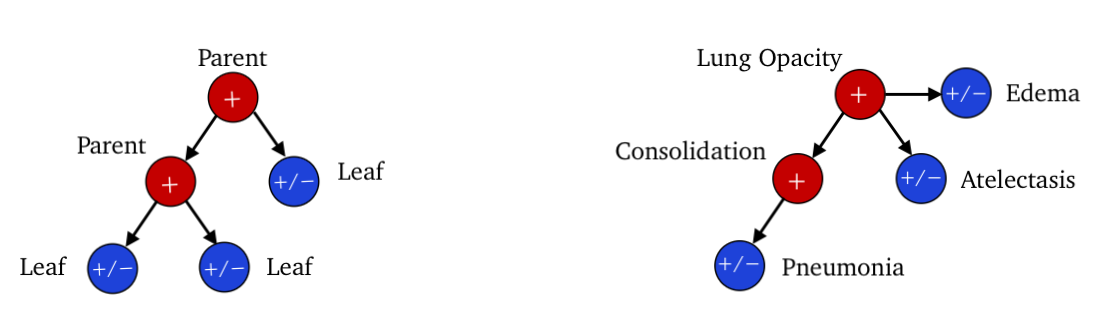
\includegraphics[scale=0.37]{Tesi/images/Conditional Training.png}
\caption[Conditional Training Example]{The left figure shows the key idea behind conditional training. In the right one there is an example, in which the classifier is trained on samples containing only positive instances of \textit{Lung Opacity} and \textit{Consolidation} in order to classify the child labels \textit{Edema}, \textit{Atelectasis} and \textit{Pneumonia}.}
\label{fig:figure_4.3}
\end{figure}

Using this training strategy, the output of the network can be viewed as the conditional probability that a label is positive giving its parent label being positive. Our goal, however, is to predict the unconditional probability. In order to do that we can rely on Bayes Theorem, calculating the probability of each label being positive by multiplying each conditional probability produced by network along the path from the root to the current node.
For example, considering the tree depicted in Figure \ref{fig:figure_4.4}, where $\boldsymbol{\alpha}$ and $\boldsymbol{\beta}$ are parent labels, while  $\boldsymbol{\gamma}$  and  $\boldsymbol{\delta}$ are leaf:

\newpage

\begin{figure}[htbp!]
\centering

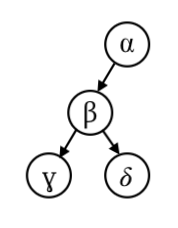
\includegraphics[scale=0.5]{Tesi/images/CT_inference.png}
\caption{Example of tree presenting four diseases}
\label{fig:figure_4.4}
\end{figure}

\noindent The network provides the conditional probabilities $p(\alpha)$, $p(\beta|\alpha)$, $p(\gamma|\beta)$, $p(\delta|\beta)$. The unconditional predictions for labels $\boldsymbol{\gamma}$  and  $\boldsymbol{\delta}$, instead, are given by: 

\begin{equation}
\begin{split}
    p(\boldsymbol{\gamma}) = p(\boldsymbol{\alpha})p(\boldsymbol{\beta}|\boldsymbol{\alpha})p(\boldsymbol{\gamma}|\boldsymbol{\beta})\\[7pt]
 p(\boldsymbol{\delta}) = p(\boldsymbol{\alpha})p(\boldsymbol{\beta}|\boldsymbol{\alpha})p(\boldsymbol{\delta}|\boldsymbol{\beta})
 \end{split}
    \label{eq:eq_4.4}
\end{equation}

\noindent Note that this approach ensures that the probability of presence of a disease for a child label is always smaller than that of its parent.

\subsection{Neural Network Ensemble}
\label{sec:nn_ensemble}
In Chapter \ref{cha:second_chapter} we have talked about Ensemble, a widely used Machine Learning technique who's aim is to gather the predictions coming from different classifiers and combine them in order to enhance the quality of the predictions.

\vspace{5mm}

In a multilabel classification setting it's hard to obtain high results for each target using a single classifier and, often, the score for each label varies with the choice of the architecture. So we decided to rely on Embedding, trying to combine several weak classifiers into a stronger one. Again, instead of building our own architecture from scratch, we used some of the most popular pretrained network emplyoed for image classification tasks. The list of the network we have used, along with some information about their structure, is shown in Table \ref{table:table_4.1}

\newpage

\begin{table}[h!]
\centering
\begin{tabular}{|l|l|l|l|l|} 
\hline
\textbf{Name}     & \textbf{\#Parameters} & \hfill\textbf{Depth} & \hfill\textbf{Size} & \hfill\textbf{Year}  \\ 
\hline
DenseNet121       & \hfill7M                    & \hfill121               &  \hfill33MB             & \hfill2016 \cite{densenet}              \\
DenseNet169       & \hfill12,5M                 & \hfill169               &   \hfill57MB            &     \hfill2016 \cite{densenet}           \\
DenseNet201       & \hfill18M                   & \hfill201              &   \hfill80MB           &        \hfill2016 \cite{densenet}        \\
InceptionResNetV2 & \hfill54M                   & \hfill572             &      \hfill215MB         &      \hfill2016 \cite{inceptionresnetv2}          \\
Xception          & \hfill21M                   &  \hfill126              &     \hfill88MB          &    \hfill2016 \cite{xception}            \\
VGG16             & \hfill15M                   &   \hfill23             &   \hfill528MB            &  \hfill2014 \cite{vgg16}               \\
VGG19             & \hfill20M                   &   \hfill26             &    \hfill549MB           &      \hfill2014 \cite{vgg16}           \\
\hline
\end{tabular}
\caption{List of pretrained CNN used}
\label{table:table_4.1}
\end{table}

All the Networks have been trained following the same approach used for the training of DenseNet121 (described in Section \ref{sec:single_cnn}). At the end of the training process, thus, we had 7 classifiers, each one carrying out a different set of predictions. We will now talk about the approaches we investigated to combine them.

\vspace{5mm}

\noindent\scalebox{1.4}{\textbf{Average}}

\vspace{2mm}

\noindent The first (and simplest) approach we have used consist in averaging the predictions made by the classifiers. If we indicate with $y_{i}(\mathbf{x})$ the 14-dimensional output of classifier $i$, then the final prediction $\tilde{y}(\mathbf{x})$, computed using the predictions coming from all the $N$ classifiers, is given by:  

\begin{equation}
    \centering
    \tilde{y}(\mathbf{x}) = \frac{1}{N}\sum_{i=1}^{N} y_{i}
    \label{eq:eq_4.5}
\end{equation}

\vspace{3mm}

\noindent The main drawback of this approach, however, is that it gives the same importance to all the models, without taking care of the fact that some classifiers may outperform other in classifying some diseases and, thus, their opinion should have a higher weight in the process of carrying out the final prediction.

\vspace{7mm}

\noindent\scalebox{1.4}{\textbf{Weighted Average}}

\vspace{2mm}

\noindent We tried to overcome the problem that arose using a simple average aggregation by using a different weight for each model. The weights have been assigned using an heuristic we developed that is based on the concept of Entropy. In Information Theory the Entropy is a quantity associated to a random variable that capture the level of uncertainty related to its possible outcome. For example, consider tossing a coin: in the case in which the coin is fair (i.e head and tail have both the same probability to occur), we are very insecure about the result, thus in this case the entropy is maximum. If, instead, the coin is not fair and one result has a higher probability to occur than the other, the result will be less uncertain and, consequently, the entropy will be lower.
We used this quantity to measure the level of uncertainty of each outcome. Consider, for example, the prediction $p_{i}$ for label $i$, taken out by a given model. We can compute the entropy of the predicions as: 

\begin{equation}
    H(p_{i}) = - p_{i} \log _{2}p_{i} - \left(1-p_{i} \right) \log _{2}\left( 1-p_{i} \right)
    \label{eq:eq_4.6}
\end{equation}

\noindent Note that, if $H(p_{i})$ captures the information related to the uncertainty of a prediction, $(1-H(p_{i}))$, instead, gives us an insight related to how safe the model is about it.

\noindent Now that we have introduced the concept of entropy we can describe how we used it in our task. Consider a \ac{CXR} given as input to our $N=7$ predictors. The output associated to the $L=14$ labels can be represented as a matrix: 

\begin{equation}
P =
\begin{bmatrix} 
    p_{11} & \dots & p_{1L} \\
    \vdots & \ddots & \vdots\\
    p_{N1} &  \dots      & p_{NL} 
\end{bmatrix}
\label{eq:eq_4.7}
\end{equation}

\noindent where $p_{ij}$ is the predictions carried out by i-th model for label $j$. Using equation \ref{eq:eq_4.6} we can also compute a matrix of weigths:

\begin{equation}
H =
\begin{bmatrix} 
    h_{11} & \dots & h_{1L} \\
    \vdots & \ddots & \vdots\\
    h_{N1} &  \dots      & h_{NL} 
\end{bmatrix}
\label{eq:eq_4.8}
\end{equation}

\vspace{4mm}

\noindent Now, the final prediction $y_{i}$ for label $i$ can be calculated as a weighted average of all the outputs, where a weight captures the certainty of the model with respect its own prediction. Here's the mathematical formulation: 

\begin{equation}
y_{i} = \sum _{k=1}^{N} \left(1- h_{ki} \right)p_{ki}
\label{eq:eq_4.9}
\end{equation}

\vspace{7mm}

\noindent\scalebox{1.4}{\textbf{Stacking}}

\vspace{2mm}

\noindent The last aggregation approach we investigated is the one involving Stacking, a technique already presented in Section \ref{sec:ensemble}. The idea is to let an algorithm learn the best way to combine the predictions instead of doing it manually. 
We have used the predictions generated over our validation set as input to train a meta-learner, who's aim is that of aggregating the outputs in order to generate the final prediction. Note that in order to train the meta-learner it's very important to use data that have not been employed during the training of the base classifiers, otherwise we would incur in overfitting.
The predictions coming from all the networks have been stacked together, thus the size of a single example was constituded by $L \times N$ data points, where $L$ is the number of labels and $N$ the number of predictors.
As meta-learner we used a Random Forest algorithm, whose hyperparameters have been tuned using a Grid Search approach.

\section{Embedding}
\label{sec:nn_embedding}
The inherent ability of \acp{CNN} to deal with images made them a standard for the task of \acp{CXR} analysis. In this section, however, we try to investigate other approaches that can be used to classify the pathologies. For many algorithms, however, it's almost impossible to learn the discriminative features directly from the image, unless it has a very small size. It would be useful, then, to have a small representation of the \ac{CXR} that, however, is able to capture all the meaningful informations nedeed by the algorithm. Neural Networks can provide us such a representation by using a technique called Embedding, presented in section \ref{sec:embedding}. When the input image is processed by the network, indeed, it pass through a sequence of layers who's aim is to extract the meaningful features that are subsequently used to feed the fully connected classifier. During this process, moreover, the image is downsampled by the pooling layer, thus its spatial size is reduced as it flows through the layers. So, if we cut the network at a certain point, the output we observe is a representation of the original input embedded into a lower dimensional space. 
In our work we have extracted the embedding using the Neural Networks we trained described in Section \ref{sec:nn_ensemble} (note that each model provided us a different embedding). All the Networks have been cut at the same point, that is immediately after the Global Average Pooling layer, producing a one-dimensional vector. Table \ref{table:table_4.2} provides an insight about the shape of the embedding for each model:


\begin{table}[h!]
\centering
\begin{tabular}{|l|l|} 
\hline
\textbf{Model Name}         &   \hfill \textbf{Embedding Shape}\\
\hline
DenseNet121 &   \hfil (1,1024) \\\hline
DenseNet169 &  \hfil (1,1664)   \\\hline
DenseNet201 &  \hfil (1,1920) \\\hline
InceptionResNetV2 &  \hfil (1,1536) \\\hline
Xception &  \hfil (1,2048) \\\hline
VGG16 &  \hfil (1,512) \\\hline
VGG19 &  \hfil (1,512) \\\hline

\end{tabular}
\caption{Embedding Shape}
\label{table:table_4.2}
\end{table}

\subsection{Random Forest}
\label{sec:random_forest_model}
Once we've extracted the embeddings, they can be used as input for other models. The first approach we have explored is that involving Random Forest. As introduced in Chapter \ref{cha:first_chapter}, Random Forest is a learning algorithm that combines a group of decision trees and aggregates their output. 
Since the embeddings we had were different from each other, we decided to train a different Random Forest for each one of them. Using the validation set, we have optimized the hyperparameters by means of a Grid Search algorithm, that is an exhaustive search through a manually specified subset of values. The following hyperparameters have been taken into consideration: 
\begin{itemize}
    \item \textbf{Number of estimators}: the number of tree in the forest. Due to computational reason it has been set 200 for all our models.
    \item \textbf{Max features}: number of features to consider when looking for the best split (for each model we set it equal to the square root of the total number of variables).
    \item \textbf{Max depth}: maximum depth of the trees. The deeper the tree, the more precise it is, but this could lead to overfitting.
    \item \textbf{Min sample split}: minimum number of samples required to split an internal node.
    \item \textbf{Min sample leaf}: minimum number of samples required to be at a leaf node.
\end{itemize}

\noindent Table \ref{table:table_4.3} contains a summary of hyperparameters we used for each model.

\begin{table}[h!]
\centering
\begin{tabular}{|l|l|l|l|l|} 
\hline
\textbf{Model Name} &   \hfil \textbf{Max Depth}&   \hfil \textbf{Min Sample Split}&   \hfil \textbf{Min Sample Leaf}\\
\hline
DenseNet121 &       \hfil15  &   \hfil2 &   \hfil10  \\\hline
DenseNet169 &       \hfil15  &   \hfil2 &   \hfil10  \\\hline
DenseNet201 &       \hfil30  &   \hfil10 &   \hfil10  \\\hline
InceptionResNetV2&  \hfil30  &   \hfil10 &   \hfil1  \\\hline
Xception    &       \hfil30  &   \hfil10 &   \hfil1  \\\hline
VGG16       &       \hfil 5  &   \hfil2 &   \hfil 10 \\\hline
VGG19       &       \hfil15  &   \hfil50 &   \hfil 1 \\
\hline
\end{tabular}
\caption{Random Forest Hyperparameters}
\label{table:table_4.3}
\end{table}


\noindent Once the models have been trained, we combined their predictions using the same approaches discussed in the previous section (simple average, weighted average with entropy and stacking).


\subsection{XGBoost}
\label{sec:xgboost_model}
The last approach we tried is the one involving XGBoost (eXtreme Gradient Boosting) \cite{xgboost}, that is an efficient implementation of Gradient Boosting, introduced in section \ref{sec:gradient_boosting}. As already mentioned, this algorithm iteratively improves the predictions, adjusting them by making a step in the direction minimizing the loss function, which is given by the gradients.
We trained a different classifier for each one of the embedding we extracted from our Neural Networks and we combined their predictions using the same approaches described in the previous section.
In order to prevent overfitting, we constrained the structure of the trees, setting the maximum depth to 3 and then we trained each models for 50 rounds. 



\section{Class Activation Map}
\label{sec:class_activation_map}
As previously stated, the goal of this work is double: predicting the probability, for a given pathology, to be present on a \ac{CXR} and also localize it. Up to this moment we focused the attention on the first task, thus we want now to talk about the second one. 
The Neural Networks we trained allowed us to extract the Class Activation Map, that is the area that the model predicts to be the most indicative of each observation.The activation maps have been generated following the methodology proposed in \cite{cam_paper} and illustrated in Section \ref{sec:cam}: given a trained \ac{CNN}, the \ac{CAM} can be computed by making a weighted sum of the feature maps extracted by the last convolutional layer. Since we trained many models, we were able to compute multiple Class Activation Maps and, as already made during the classification task, combine them in order to improve the quality. However it would have made no sense to aggregate indiscriminately all of them, because we would risk to combine a map produced by a model predicting the absence of a pathology with one coming from a model telling the opposite. Thus we have decided to merge only the heatmaps coming from models having the same prediction over the presence or absence of the disease. 

\subsection{Bounding Box Generation}
\label{sec:bounding_box}
Once we have generated the \ac{CAM}, we used them to automatically generate a bounding box surrounding the area associated to the pathology. In order to do that, we first used the Class Activation Map as a mask to determine the salient area of the image. In order to do that, we have converted each pixel of the \ac{CAM} to a binary value, using the following rule:
\begin{equation}
    b(x,y) = \left\{\begin{matrix}
1, & \textup{if CAM(x,y)} \geq  threshold 
\\ 
0, & \textup{if CAM(x,y)} < threshold 
\end{matrix}\right.
\label{eq:cam_mask}
\end{equation}

where $b(x,y)$ is the intensity value of a pixel at position $(x,y)$. The threshold, instead, has been computed as:

\begin{equation}
   threshold = \alpha \times max(\textup{CAM}), \alpha \in \left[0,1\right]
   \label{eq:threshold}
\end{equation}

Once we got the mask, it has been overlapped to the original image $I$, and the saliency region $p(x,y)$ has been extracted by making a pointwise product:

\begin{equation}
  p(x,y) = I(x,y) \cdot b(x,y)
   \label{eq:saliency_region}
\end{equation}

Once we got that image, we were able to extract the coordinates of its contours and, using them, we draw the bounding box over the original image. Figure \ref{fig:figure_4.5} shows the full process used to automatically extract the bounding box. The first figure contains the original \ac{CXR}, the second one shows the generated \ac{CAM}, the third one represents the saliency region $p(x,y)$ extracted using the heatmap and, finally, the last one shows the automatically generated bounding box.

\begin{figure}[htbp!]
\centering
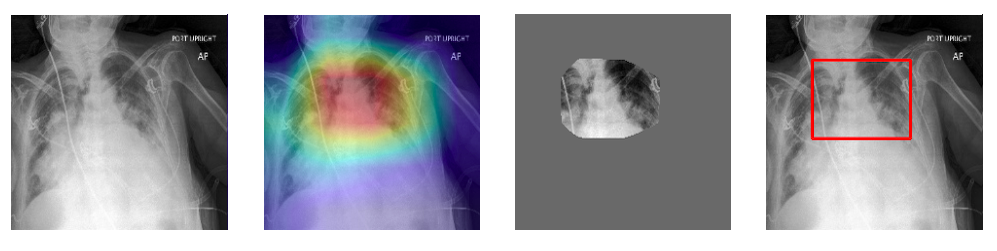
\includegraphics[scale=0.43]{Tesi/images/bbox.png}
\caption{Bounding Box Generation}
\label{fig:figure_4.5}
\end{figure}

\section{Summary}
\label{sec:chapter_4_summary}
In this chapter we have shown all the techniques we have used to solve the problems of predicting and localizing the different diseases. We started showing how to better deal with the uncertain labels, then we have built the first model that, gradually, we have modified, trying to improve the overall predictions perfomances. Finally we have shown the ability of the trained models to localize the pathologies on the \ac{CXR} and how this localization ability can be used to automatically generate a bounding box sorrounding the region interested by the pathology. In the next chapter we will talk about the metrics we used to evaluate our models and we'll exhibit and discuss the results we achieved.
\chapter{Results}
\label{cha:fifth_chapter}
In this chapter we will first introduce the methodology we used to evaluate our models and then we will show and discuss the results we have obtained both in classifying the diseases and in localizing them. 

\section{Evaluation Criteria}
\label{sec:evaluation_criteria}
As introduced in Chapter \ref{cha:third_chapter}, the dataset already provides a subset of 202 frontal images that can be used to asses the performances of the models. We decided, in our work, to evaluate our models using the same subset, in order to be able to compare our results with that carried out by related works.
The performance, however, have not been evaluated over the entire set of pathologies but, instead, only 5 of them (\textit{Atelectasis}, \textit{Cardiomegaly}, \textit{Consolidation}, \textit{Edema}, \textit{Pleural Effusion}) have been taken into consideration, based on their clinical significance and presence in the dataset. 

\subsubsection{AUROC}
\ac{AUROC} is the summary metric we used to assess the goodness of our classifiers. In order to define it, we have to first introduce some quantities that are largely used to measure the performance of a classifier:
\begin{itemize}
    \item \ac{TP}: outcome \textit{correctly} classified as \textit{positive}
    \item \ac{TN}: outcome \textit{correctly} classified as \textit{negative}
    \item \ac{FP}: outcome \textit{incorrectly} classified as \textit{positive}
    \item \ac{FN}: outcome \textit{incorrectly} classified as \textit{negative}
\end{itemize}

We can now introduce the notion of Receiving Operating Characteristic, that is a curve plotting the \ac{TPR} against the \ac{FPR}. \ac{TPR}, also known as sensitivity or recall, measures the proportion of actual positive that are identified as such, and is computed as:
\begin{equation}
\textup{TPR} = \frac{\textup{TP}}{\textup{TP + FN}}
    \label{eq:equation_5.1}
\end{equation}

\ac{FPR}, instead, measures the probability of a false alarm, i.e the number of negative samples incorrectly classified as positive, and is given by: 
\begin{equation}
\textup{FPR} = \frac{\textup{FP}}{\textup{FP + TN}}
    \label{eq:equation_5.1}
\end{equation}

In order to compute these quantities, however, the predictions, that are expressed as probabilities, must be converted into binary decisions, in other words a value telling whether a given sample is classified as positive or negative. This can be done by defining a value of the probability, called decision threshold, above which the samples are classified as positive while, otherwise, they are assigned to the negative class. Once a threshold value has been selected, the performance of a classifier can be represented as a point in the ROC space. Consider, for example, Figure \ref{fig:figure_5.1}:
\vspace{5mm}
\begin{figure}[htbp!]
    \centering
    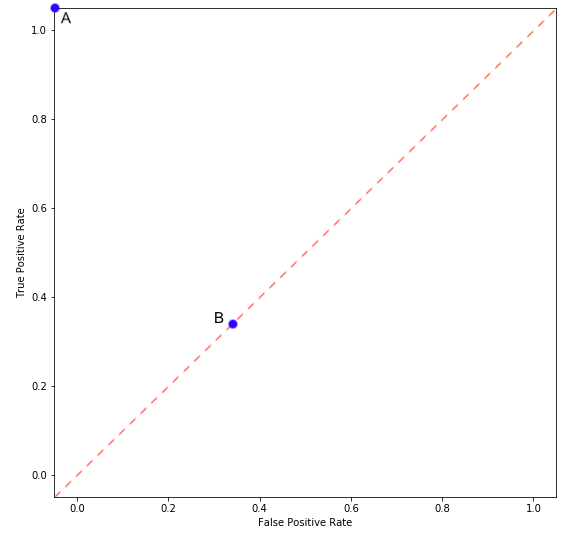
\includegraphics[scale=0.45]{Tesi/images/ROC.png}
    \caption{ROC Example}
    \label{fig:figure_5.1}
\end{figure}

\newpage
Point $\textup{A=(0,1)}$ represents the ideal case, in which all the samples are assigned to the correct class. Point $\textup{B}$, instead, lies on the so called \textit{line of no discrimination}, whose performance is the same of a random guessing. Note that the line of no discrimination splits the ROC space into two parts: points above the line represents good classification results, while points below represents bad results (worse than random).
A way to asses the overall performance of a predictor is that of drawing a curve on the ROC plane by plotting its score for every possible threshold value used to discriminate between positive and negative class. Then we can finally calculate the area under the curve, obtaining the \ac{AUROC} value (also called AUC). For what it concern the medical field,according to \cite{auroc}, an AUC of 0.5 suggests no discrimination, 0.7 to 0.8 is considered acceptable, 0.8 to 0.9 is considered excellent, and more than 0.9 is considered outstanding.

\vspace{5mm}
\section{Experimental Design}
\label{sec:experimental_design}
The first experiment we conducted involved a single CNN, more specifically a DenseNet121. Using U-Ones as policy for dealing with uncertain labels, we trained it for 5 epochs using a training set composed by 189116 samples. The learning rate was initially set to 1e-4 and then reduced by a factor of 10 after each epoch. As objective function we used the binary cross-entropy. Then we have repeated the experiment but using U-Ones+LSR as policy for dealing with uncertain labels.
\noindent Next step was that of exploiting the diseases taxonomy, using Conditional Training. During the first phase we used a training set composed by 90954 samples and we trained the DenseNet121 network end to end, using the same set up of the previous experiments. Then we froze all the layers except the last fully connected one and we retrain the network using all the 189116 samples for 5 epochs. The same procedure has been repeated for each architecture indicated in Table \ref{table:table_4.1}, obtaining the 7 different models that we then combined exploiting different ensemble techniques.
Moreover, the networks have been used to generate the embeddings, extracted from the Global Average Pooling layer and then used to train both Random Forest and XGBoost. The hyperparameters have been tuned using a validation set composed by 1911 samples. 


\section{Experiment Results}
\label{sec:experiment_result}

We will now present and discuss the results we obtained in our experiments, using the models we have introduces in the previous chapter. We will compare each other, showing, for each one, the benefits and the downsides.

\vspace{5mm}

\subsection{Single CNN}
Our first objective was to check the effectiveness of Label Smooth Regularization and Conditional Training. Starting from a simple model, that we used as baseline, we then implemented the two strategies, checking whether they were able to bring some improvements or not.
As baseline we used a DenseNet121 architecture (the same used in \cite{irvin2019chexpert} \cite{pham2019interpreting}), trained with U-Ones policy for dealing with uncertain labels. As we can see in Figure \ref{fig:figure_5.2}, this approach was able to achieve a mean AUROC across the five diseases of 0.865 which, according to \cite{auroc}, is already a good result. The network, however, showed difficulties in recognizing the cases of Atelectasis and Cardiomegaly, while, instead, was able to identify pretty well the \acp{CXR} containing Edema and Pleural Effusion that, is worth noting, are the most balanced diseases among those we are considering (Table \ref{table:table_2}).

\begin{figure}[htbp!]
    \centering
    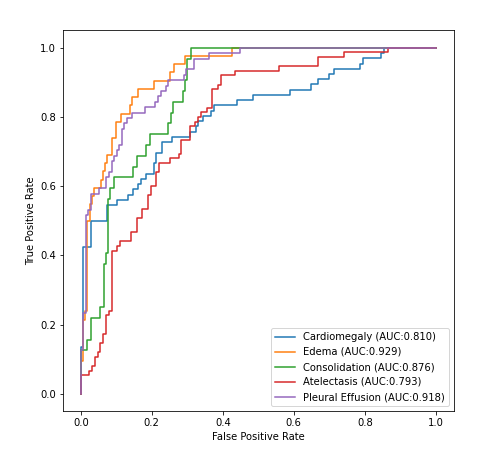
\includegraphics[scale=0.57]{Tesi/images/Results/densenet121_baseline.png}
    \caption[ROC curve for U-Ones policy]{ROC curve of DenseNet121 architecture trained with U-Ones policy}
    \label{fig:figure_5.2}
\end{figure}

\newpage

Using the Label Smooth Regularization, together with the U-Ones policy, led to an improvement in recognizing all the pathologies except for Consolidation, where the previous approach outperformed the current one (Figure \ref{fig:figure_5.3}).

\begin{figure}[htbp!]
    \centering
    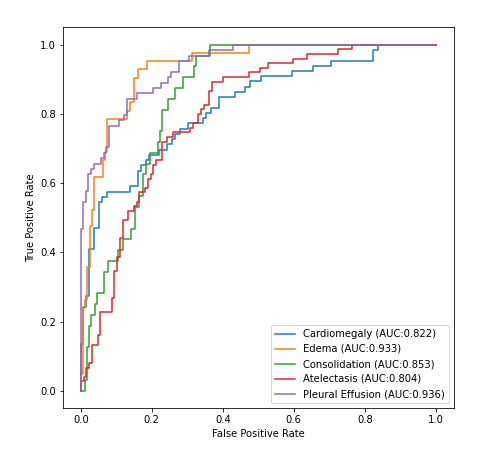
\includegraphics[scale=0.55]{Tesi/images/Results/densenet121_LSR (1).png}
    \caption[ROC curve for U-Ones+LSR policy]{ROC curve of DenseNet121 trained with U-Ones policy + Label Smooth Regularization.}
    \label{fig:figure_5.3}
\end{figure}


The use of Conditional Training, instead, gave a big improvement in identifying the cases of Atelectasis and Consolidation (Figure \ref{fig:figure_5.4}), with the downside of slightly worsening the performance over the other diseases. The mean \ac{AUROC}, however, is the best obtained so far (0.876), confirming the hypothesis that using additional side information, such as dependencies among the pathologies, can help improving the overall performance of the network.
\newpage
\begin{figure}[htbp!]
    \centering
    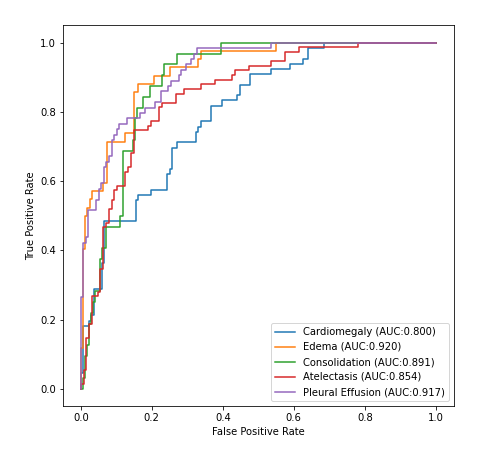
\includegraphics[scale=0.55]{Tesi/images/Results/densenet121_LSR_CT.png}
    \caption[ROC curve for U-Ones+LSR+CT policy]{ROC Curve of DenseNet121 trained with U-Ones policy + Label Smooth Regularization + Conditional Training.}
    \label{fig:figure_5.4}
\end{figure}

\vspace{5mm}

Table \ref{table:table_5.1} shows the comparison of the three different approaches we've investigated using a single CNN.

\begin{table}[h!]
\centering
\resizebox{\columnwidth}{!}{
\renewcommand{\arraystretch}{1.5}
\begin{tabular}{|l|l|l|l|l|l|l|} 
\hline
\textbf{Method} & \textbf{Atelectasis} & \textbf{Cardiomegaly} & \textbf{Consolidation} & \textbf{Edema} & \textbf{P.}~\textbf{Effusion} & \textbf{Mean}  \\
\hline
U-Ones& 0.793 & 0.810  & 0.876 & 0.929 & 0.918 & 0.865\\\hline

U-Ones+LSR & 0.804 & \textbf{0.822}  & 0.853 & \textbf{0.933} & \textbf{0.936} & 0.869\\\hline

U-Ones+LSR+CT & \textbf{0.854} & 0.800  & \textbf{0.891} & 0.920 & 0.917 & \textbf{0.876}\\ 
\hline
\end{tabular}
}
\caption[AUROC comparison for different training policies on DenseNet121]{AUROC values obtained using DenseNet121 as architecture and the approaches indicated in the \textbf{Method} column. For each label, the highest AUROC is boldfaced.}
\label{table:table_5.1}
\end{table}



\subsection{CNN Ensemble}

 Table \ref{table:table_5.2} shows the results achieved by the other \ac{CNN} architectures trained using U-Ones+LSR+CT policy. The mean \acp{AUROC} are very similar among each other and they all present analogous behaviour in distinguishing the individual diseases: the greatest difficulties are encountered while recognizing the cases of Cardiomegaly, while they all achieve the best results identifying Edema and Pleural Effusion. The results we obtained confirm the fact that there is no an architecture outperforming all the others on each pathology. Consider, for example, the VGG19 network: it achieved the best result in recognizing Consolidation and Pleural Effusion but, instead, its performance on Cardiomegaly is the worst. 

\begin{table}[h!]
\centering
\resizebox{\columnwidth}{!}{
\renewcommand{\arraystretch}{1.5}
\begin{tabular}{|l|l|l|l|l|l|l|} 
\hline
\textbf{Model} & \textbf{Atelectasis} & \textbf{Cardiomegaly} & \textbf{Consolidation} & \textbf{Edema} & \textbf{P.}~\textbf{Effusion} & \textbf{Mean}  \\
\hline
DenseNet121& \textbf{0.854} & \textbf{0.800}  & 0.891 & 0.920 & 0.917 & \textbf{0.876}\\ \hline

DenseNet169& 0.850 & 0.795  & 0.882 & \textbf{0.936} & 0.915 & \textbf{0.876}\\ \hline

DenseNet201& 0.834 & 0.791  & 0.881 & 0.917 & 0.925 & 0.870\\ \hline

InceptionResNetV2& 0.816 & 0.784  & 0.897 & 0.925 & 0.919 & 0.869\\ \hline

Xception& 0.841 & 0.770  & 0.880 & 0.909 & 0.924 & 0.865\\ \hline

VGG16& 0.843 & 0.772  & 0.898 & 0.932 & 0.919 & 0.873\\ \hline

VGG19& 0.843 & 0.769  & \textbf{0.900} & 0.927 & \textbf{0.933} & 0.874\\ \hline

\end{tabular}
}
\caption[\acp{CNN} AUROC results]{AUROC values obtained with the \acp{CNN} indicated in the \textbf{Model} column.}
\label{table:table_5.2}
\end{table}

Once we trained the different networks, we tried to improve the overal diagnostic capability by combining them. Figures \ref{fig:figure_5.5} and \ref{fig:figure_5.6} show, respectively, the results of applying simple Average and Entropy Weighted Average as aggregation methods.  As we can see, both the approaches helped improving the model's ability to recognize each of the five pathologies. More specifically, as we can see from Table \ref{table:table_5.3}, making an entropy weighted average that took care of each model's accuracy turned out to be a successful aggregation strategy, leading to a mean \ac{AUROC} of 0.889, a result that slightly outperformed the simple average approach. 



\begin{figure}[htbp!]
    \centering
    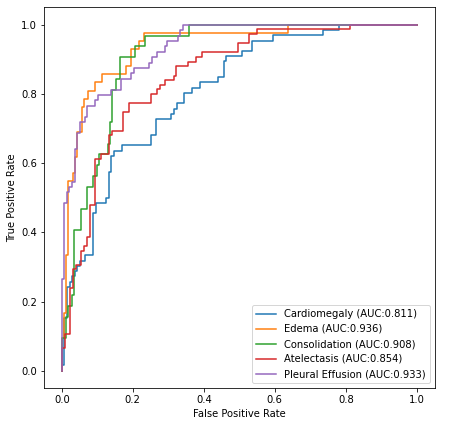
\includegraphics[scale=0.55]{Tesi/images/Results/nn_average.png}
    \caption[ROC curve for CNN average ensemble]{ROC curve of the \acp{CNN} ensemble  computed using simple average.}
    \label{fig:figure_5.5}
\end{figure}

\begin{figure}[htbp!]
    \centering
    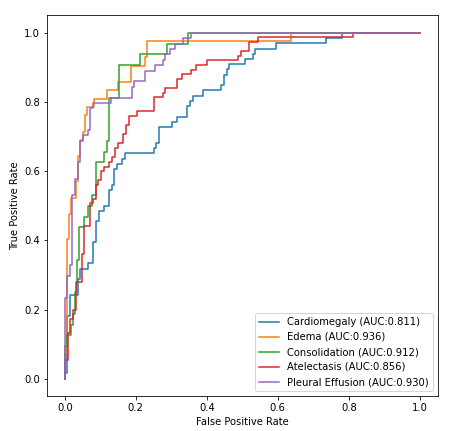
\includegraphics[scale=0.55]{Tesi/images/Results/nn_average_entropy.png}
    \caption[ROC curve for CNN weighted average ensemble]{ROC curve of the \acp{CNN} ensemble model computed using average weighted by predictions' entropy.}
    \label{fig:figure_5.6}
\end{figure}

\newpage

An aggregation approach based on Stacking, however, didn't boost the overall performance, leading to a significant improvement only in Pleural Effusion recognition.

\begin{figure}[htbp!]
    \centering
    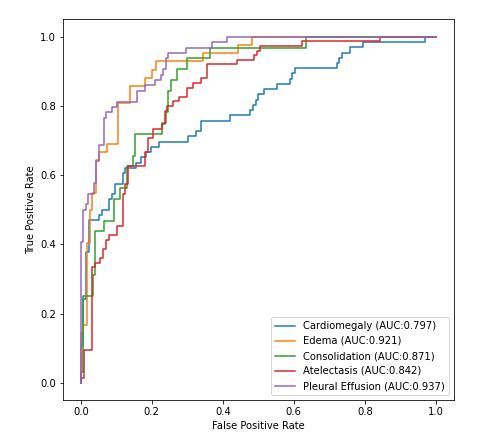
\includegraphics[scale=0.55]{Tesi/images/Results/nn_stacking.png}
    \caption[ROC curve for CNN stacking ensemble]{ROC curve of the \acp{CNN} ensemble model computed using stacking.}
    \label{fig:figure_5.7}
\end{figure}

Table \ref{table:table_5.3} reports the \acs{AUROC} obtained by the three ensemble policies, compared to the best results achieved using a single \ac{CNN}. We can clearly see that aggregating the predictions led to a significant improvement. In particular, making an entropy weighted average that took care of each model's accuracy turned out to be a successful aggregation strategy, leading to a mean \ac{AUROC} of 0.889, a result that slightly outperformed the simple average approach. 


\begin{table}[h!]
\centering
\resizebox{\columnwidth}{!}{
\renewcommand{\arraystretch}{1.5}
\begin{tabular}{|l|l|l|l|l|l|l|} 
\hline
\textbf{Method} & \textbf{Atelectasis} & \textbf{Cardiomegaly} & \textbf{Consolidation} & \textbf{Edema} & \textbf{P.}~\textbf{Effusion} & \textbf{Mean}  \\
\hline
Single CNN& 0.854 &0.800  & 0.900 & \textbf{0.936} & 0.933 & 0.885\\\hline

Average Ensemble& 0.854 & \textbf{0.811}  & 0.908 & \textbf{0.936} & 0.933 & 0.888\\\hline

Entropy Weighted AVG & \textbf{0.856} & \textbf{0.811}  & \textbf{0.912} & \textbf{0.936} & 0.930 & \textbf{0.889}\\\hline

Stacking & 0.842 & 0.797  & 0.871 & 0.921 & \textbf{0.937} & 0.873\\\hline

\end{tabular}
}
\caption[\acp{CNN} ensemble AUROC comparison]{AUROC values obtained using different Ensemble policies, compared to the best results achieved by a single CNN (reported in the first row). For each label, the highest AUROC is boldfaced.}
\label{table:table_5.3}
\end{table}


\subsection{Random Forest with Embedding}
\label{sec:rf_embedding_results}


Once we trained the \acp{CNN}, we used them to extract the embeddings. The first algorithm we used exploting them is Random Forest, whose results are shown in the Table \ref{table:table_5.4}.

\begin{table}[h!]
\centering
\resizebox{\columnwidth}{!}{
\renewcommand{\arraystretch}{1.5}
\begin{tabular}{|l|l|l|l|l|l|l|} 
\hline
\textbf{Model} & \textbf{Atelectasis} & \textbf{Cardiomegaly} & \textbf{Consolidation} & \textbf{Edema} & \textbf{P.}~\textbf{Effusion} & \textbf{Mean}  \\
\hline
DenseNet121& 0.851 & \textit{0.818}  & 0.885 & 0.915 & \textbf{\textit{0.945}} & \textit{0.883}\\ \hline

DenseNet169& \textit{0.855} & \textit{0.814}  & \textit{0.893} & \textbf{0.922} & \textit{0.933} & \textbf{\textit{0.884}}\\ \hline

DenseNet201& \textit{0.863} & \textit{0.814}  & 0.878 & \textbf{\textit{0.922}} & \textit{0.936} & \textit{0.882}\\ \hline

InceptionResNetV2& \textit{0.830} & 0.779  & \textit{0.898} & 0.918 & \textit{0.933} & \textit{0.872}\\ \hline

Xception& 0.831 & \textit{0.810}  & \textit{0.907} & \textit{0.913} & \textit{0.932} & \textit{0.879}\\ \hline

VGG16& \textit{0.858} & \textbf{\textit{0.822}}  & \textbf{\textit{0.913}} & 0.886 & 0.917 & \textit{0.879}\\ \hline

VGG19& \textbf{\textit{0.873}} & \textit{0.798}  & 0.895 & 0.892 & 0.917 & \textit{0.875}\\ \hline

\end{tabular}
}
\caption[Random Forest AUROC results]{AUROC values obtained with Random Forest trained using the embedding extracted from the CNN indicated in the \textbf{Model} column. For each label, the highest AUROC is boldfaced. A score written in italics means that the RF, on that label, outperformed the result achieved by its corresponding CNN, reported in Table \ref{table:table_5.2}}
\label{table:table_5.4}
\end{table}


\noindent As we can see, each of the single models we trained achieved, on average, a better result than its corresponding one (shown in Table \ref{table:table_5.2}), confirming the fact that the embeddings are actually able to capture the relevant information needed to distinguish the different diseases. 


\noindent As in the previous case, we combined the predictions carried out by the different models, investigating the same approaches used before. Figures \ref{fig:figure_5.8} and \ref{fig:figure_5.9} show the results obtained using, respectively, Average and Entropy Weighted Average as ensemble policy. 

\begin{figure}[htbp!]
    \centering
    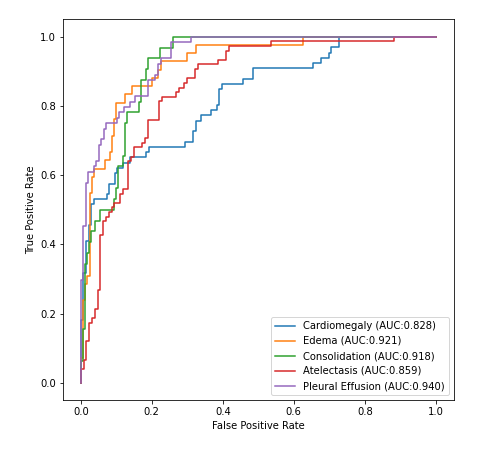
\includegraphics[scale=0.55]{Tesi/images/Results/rf_average.png}
    \caption[ROC curve for RF simple average ensemble]{ROC curve of the RF ensemble model computed using simple average.}
    \label{fig:figure_5.8}
\end{figure}

\begin{figure}[htbp!]
    \centering
    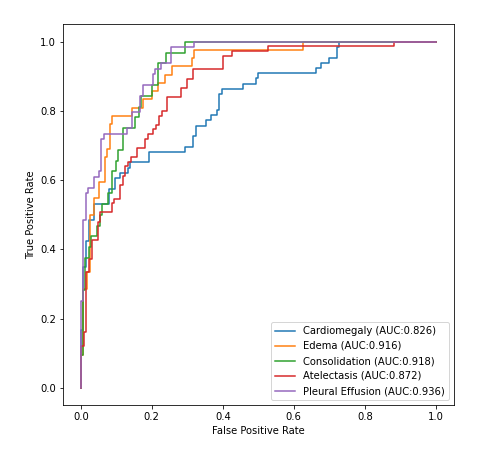
\includegraphics[scale=0.55]{Tesi/images/Results/rf_average_entropy.png}
    \caption[ROC curve for RF weighted average ensemble]{ROC curve of the RF ensemble model computed using average weighted by predictions' entropy.}
    \label{fig:figure_5.9}
\end{figure}

\noindent They both brought to a significant improvement, with the latter achieving a mean AUROC of 0.897 (Table \ref{table:table_5.5}), the highest result among those we have seen so far. 

\noindent Using stacking as aggregation method, instead, didn't help improving the diagnosis. On the contrary, this approach drastically reduced the performance on Cardiomegaly, leading to one of the worst score on that label. 

\begin{figure}[htbp!]
    \centering
    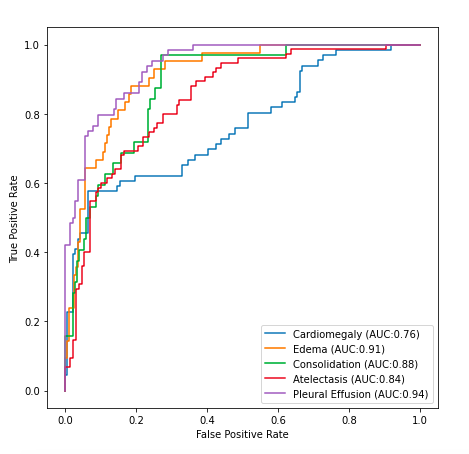
\includegraphics[scale=0.55]{Tesi/images/Results/rf_stacking.png}
    \caption[ROC curve for RF stacking ensemble]{ROC curve of the RF ensemble model computed using stacking.}
    \label{fig:figure_5.11}
\end{figure}

We can see the results of the three ensemble methods in Table \ref{table:table_5.5}, compared to the best result achieved by a single Random Forest (the one obtained by using the embedding extracted by the DenseNet169 architecture).


\begin{table}[h!]
\centering
\resizebox{\columnwidth}{!}{
\renewcommand{\arraystretch}{1.5}
\begin{tabular}{|l|l|l|l|l|l|l|} 
\hline
\textbf{Method} & \textbf{Atelectasis} & \textbf{Cardiomegaly} & \textbf{Consolidation} & \textbf{Edema} & \textbf{P.}~\textbf{Effusion} & \textbf{Mean}  \\
\hline
Single RF& 0.855 & 0.814  & 0.893 & 0.922 & 0.933 & 0.884\\\hline

Average& 0.859 & \textbf{0.828}  & \textbf{0.918} & \textbf{0.921} & \textbf{0.940} & 0.893\\\hline

Entropy Weighted AVG& \textbf{0.872} & 0.826  & \textbf{0.918} & 0.916 & 0.936 & \textbf{0.897}\\\hline

Stacking& 0.840 & 0.761  & 0.883 & 0.908 & 0.937 & 0.866\\\hline

\end{tabular}
}
\caption[\ac{RF} ensemble AUROC comparison]{AUROC values obtained using different Ensemble policies combining Random Forest models trained using the embeddings. For each label, the highest AUROC is boldfaced.}
\label{table:table_5.5}
\end{table}

Table \ref{table:table_5.6}, instead, shows the comparison between the best result achieved using Neural Networks with respect to that obtained by the embeddings. As we can clearly see, the latter is able to outperform the ensemble of \acp{CNN} in the recognition of all the diseases except for Edema.

\begin{table}[h!]
\centering
\resizebox{\columnwidth}{!}{
\renewcommand{\arraystretch}{1.5}
\begin{tabular}{|l|l|l|l|l|l|l|} 
\hline
\textbf{Method} & \textbf{Atelectasis} & \textbf{Cardiomegaly} & \textbf{Consolidation} & \textbf{Edema} & \textbf{P.}~\textbf{Effusion} & \textbf{Mean}  \\
\hline
CNNs& 0.856 & 0.811  & 0.912 & \textbf{0.936} & 0.930 & 0.889\\\hline

RF Embeddding& \textbf{0.872} & \textbf{0.826}  & \textbf{0.918} & 0.916 & \textbf{0.936} &  \textbf{0.897}\\\hline
\end{tabular}
}
\caption[CNNs and RF Embedding comparison]{AUROC values comparison between CNNs and RFs trained using embedding. For each label, the highest AUROC is boldfaced.}
\label{table:table_5.6}
\end{table}


\subsection{XGBoost}

The embeddings have been used to trained another set of models, based on XGBoost, whose results are reported in Table \ref{table:table_5.6}. All of them, except for DenseNet201, achieved results similar to those obtained with the \acp{CNN}. Random Forest, thus, seems to be more capable of exploiting the embedding to classify the \ac{CXR}.



\begin{table}[h!]
\centering
\caption[XGBoost AUROC results]{AUROC values obtained with XGBoost trained using the embedding extracted from the CNN indicated in the \textbf{Model} column.}
\resizebox{\columnwidth}{!}{
\renewcommand{\arraystretch}{1.5}
\begin{tabular}{|l|l|l|l|l|l|l|} 
\hline
\textbf{Model} & \textbf{Atelectasis} & \textbf{Cardiomegaly} & \textbf{Consolidation} & \textbf{Edema} & \textbf{P.}~\textbf{Effusion} & \textbf{Mean}  \\
\hline
DenseNet121& 0.803 & \textit{0.837}  & 0.837 & \textbf{\textit{0.944}} & \textit{0.935} & 0.871\\ \hline

DenseNet169& 0.812 & \textit{0.829}  & 0.866 & 0.916 & \textit{0.923} & 0.869\\ \hline

DenseNet201& \textbf{0.824} & \textbf{\textit{0.867}}  & 0.876 & \textit{0.920} & \textbf{\textit{0.938}} & \textbf{\textit{0.885}}\\ \hline

InceptionResNetV2& \textit{0.820} & \textit{0.792}  &\textbf{\textit{0.911}} & 0.911 & \textit{0.922} & \textit{0.871}\\ \hline

Xception& 0.803 & \textit{0.804}  & \textit{0.901} & 0.899 & 0.923 & \textit{0.866}\\ \hline

VGG16& \textit{0.800} & 0.840 & 0.849 & 0.922 & \textit{0.927} & 0.868\\ \hline

VGG19& 0.811 & \textit{0.819}  & 0.832 & 0.921 & 0.922 & 0.861\\ \hline

\end{tabular}
}
\label{table:table_5.7}
\end{table}

Combining the XGBoost models, however, the performance increased significantly with respect to using the single models alone (Figure \ref{fig:figure_5.11} and \ref{fig:figure_5.12}). In particular, differently from the previous approaches, by combining the XGBoost predictions the system is able to achieve good results also on Cardiomegaly that, according to the previous results, was one of the most difficult pathology to identify.


\begin{figure}[htbp!]
    \centering
    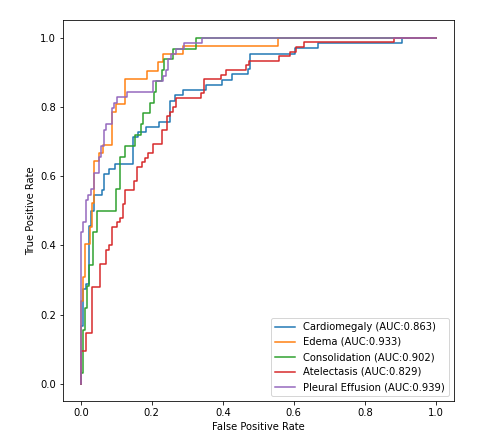
\includegraphics[scale=0.55]{Tesi/images/Results/xgb_average.png}
    \caption[ROC curve for XGBoost simple average ensemble]{ROC curve of the XGBoost ensemble model computed using simple average.}
    \label{fig:figure_5.11}
\end{figure}

\newpage

\begin{figure}[t!]
    \centering
    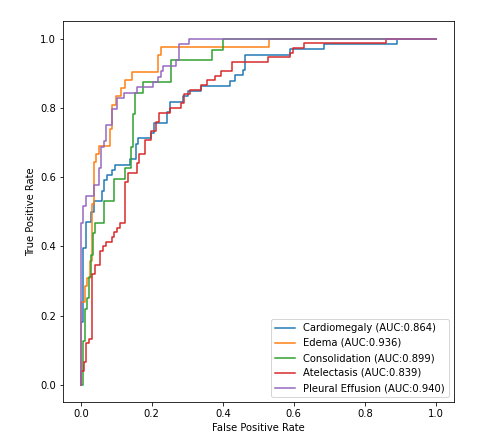
\includegraphics[scale=0.55]{Tesi/images/Results/xgb_average_entropy.png}
    \caption[ROC curve for XGBoost weighted average ensemble]{ROC curve of the XGBoost ensemble model computed using average weighted by predictions' entropy.}
    \label{fig:figure_5.12}
\end{figure}

The results obtained after the aggregation are summarized in the Table \ref{table:table_5.8}, along with the best result obtained using \acs{CNN}. Again, the use of the embedding is able to outperform the results achieved using the full images.

\begin{table}[h!]
\centering
\resizebox{\columnwidth}{!}{
\renewcommand{\arraystretch}{1.5}
\begin{tabular}{|l|l|l|l|l|l|l|} 
\hline
\textbf{Method} & \textbf{Atelectasis} & \textbf{Cardiomegaly} & \textbf{Consolidation} & \textbf{Edema} & \textbf{P.}~\textbf{Effusion} & \textbf{Mean}  \\
\hline
CNNs& \textbf{0.856} & 0.811  & \textbf{0.912} & \textbf{0.936} & 0.930 & 0.889\\\hline

XGB Average& 0.829 & 0.863  & 0.902 & 0.933 & 0.939 & 0.893\\\hline

XGB Entropy Weighted AVG& 0.839 & \textbf{0.864}  & 0.899 & \textbf{0.936} & \textbf{0.940} & \textbf{0.896}\\\hline

\end{tabular}
}
\caption[CNNs and XGBoost ensemble AUROC comparison]{AUROC values obtained using different Ensemble policies combining XGBoost models trained using the embeddings. For each label, the highest AUROC is boldfaced.}
\label{table:table_5.8}
\end{table}



\subsection{Final Results}

The final predictions have been obtained by making a simple average of the three different ensembles (CNN, RF and XGBoost), each one computed using a weighted average ensemble policy and trained using U-Ones+LSR+CT. In Figure \ref{fig:figure_5.13} are reported the ROCs curve obtained, one for each pathology.

\begin{figure}[h!]
    \centering
    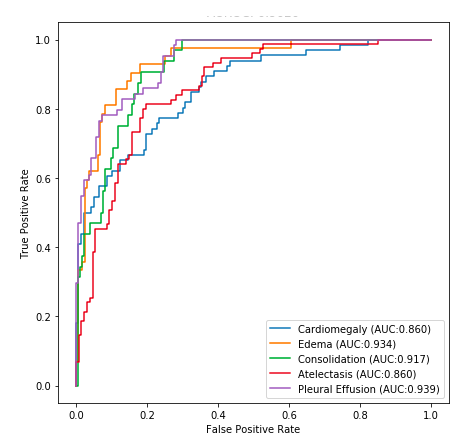
\includegraphics[scale=0.55]{Tesi/images/Results/Final Model.png}
    \caption[Final model ROC]{ROC curve of the final model, obtained by aggregating the ensembling of CNN, RF and XGBoost.}
    \label{fig:figure_5.13}
\end{figure}


Table \ref{table:table_5.9}, finally, reports a summary of all the results we obtained so far, showing the model from which we started (DenseNet121+U-Ones), the best models obtained using CNNs, RFs and XGBoost (trained using U-Ones+LSR+CT), their ensemble (obtained using Entropy Weighted Average as ensemble policy) and the final model, that achieved a mean AUROC of 0.902. The biggest improvement, with respect to the starting point, is the one involving Atelectasis and Cardiomegaly, that are the diseases on which the initial model performed worse. 

\begin{table}[h!]
\centering
\resizebox{\columnwidth}{!}{
\renewcommand{\arraystretch}{1.5}
\begin{tabular}{|l|l|l|l|l|l|l|} 
\hline
\textbf{Method} & \textbf{Atelectasis} & \textbf{Cardiomegaly} & \textbf{Consolidation} & \textbf{Edema} & \textbf{P.}~\textbf{Effusion} & \textbf{Mean}  \\
\hline
DenseNet121 + U-Ones& 0.793 & 0.810  & 0.876 & 0.929 & 0.918 & 0.865\\\hline

CNN (DenseNet121)& 0.854 & 0.800  & 0.891 & 0.920 & 0.917 & 0.876\\\hline


RF (DenseNet169)& 0.855 & 0.814  & 0.893 & 0.922 & 0.933 & 0.884\\\hline

XGB (DenseNet201)& 0.824 & \textbf{0.867}  & 0.876 & 0.920 & 0.938 & 0.885\\ \hline

CNN Ensemble& 0.855 & 0.811  & 0.912 & 0.936 & 0.930 & 0.889\\\hline

RF Ensemble& \textbf{0.872} & 0.826  & \textbf{0.918} & 0.916 & 0.936 & 0.897\\\hline

XGB Ensemble& 0.839 & 0.864  & 0.899 & \textbf{0.936} & \textbf{0.940} & 0.896\\\hline

\rowcolor[rgb]{0.851,0.851,0.851}Final Ensemble& 0.860 & 0.860  & 0.917 & 0.934 & 0.939 & \textbf{0.902}\\\hline

\end{tabular}
}
\caption[Final AUROC]{AUROC comparison of the different approaches investigated in this work. Note that, for the single models, we reported only the one achieving the highest mean result (the name of the corresponding architecture is reported between brackets).}
\label{table:table_5.9}
\end{table}

\newpage
Our final model was able to outperform, on average, the one proposed by the author of the Chexpert dataset \cite{irvin2019chexpert}, whose results are shown in the Table \ref{table:table_5.10}

\begin{table}[h!]
\centering
\resizebox{\columnwidth}{!}{
\renewcommand{\arraystretch}{1.5}
\begin{tabular}{|l|l|l|l|l|l|l|} 
\hline
\textbf{Model} & \textbf{Atelectasis} & \textbf{Cardiomegaly} & \textbf{Consolidation} & \textbf{Edema} & \textbf{P.}~\textbf{Effusion} & \textbf{Mean}  \\
\hline
Chexpert& 0.821 & 0.854  & \textbf{0.937} & 0.928 & 0.936 & 0.895\\\hline

Ours& \textbf{0.860} & \textbf{0.860}  & 0.917 & \textbf{0.934} & \textbf{0.939} & \textbf{0.902}\\\hline
\end{tabular}
}
\caption[Chexpert AUROC comparison]{AUROC comparison with Chexpert author's model (for simplicity we only report, among the results they obtained, the one with the highest mean AUROC).}
\label{table:table_5.10}
\end{table}

We weren't able, however, to outperform the system developed by Pham et al. \cite{pham2019interpreting}, whose results are reported in Table \ref{table:table_5.11}. Nevertheless we achieved good results using different approaches and, in particular, we show that using the embedding is possible to develop a \ac{CXR} diseases classifier using algorithm that are computationally much less expensive than \acp{CNN}.


\begin{table}[h!]
\centering
\resizebox{\columnwidth}{!}{
\renewcommand{\arraystretch}{1.5}
\begin{tabular}{|l|l|l|l|l|l|l|} 
\hline
\textbf{Model} & \textbf{Atelectasis} & \textbf{Cardiomegaly} & \textbf{Consolidation} & \textbf{Edema} & \textbf{P.}~\textbf{Effusion} & \textbf{Mean}  \\
\hline
Ours& 0.860 & 0.860  & 0.917 & 0.934 & 0.939 & 0.902\\\hline

Pham et al.& \textbf{0.909} & \textbf{0.910}  & \textbf{0.957} & \textbf{0.958} & \textbf{0.964} & \textbf{0.940}\\\hline

\end{tabular}
}
\caption[Pham et al. AUROC comparison ]{AUROC comparison with Pham et al. model.}
\label{table:table_5.11}
\end{table}

\subsubsection{Confusion Matrices}

Figure \ref{fig:figure_5.14} shows the confusion matrices for the five diseases, a more intuitive way to display the output of our model. For each pathology we used a different decision threshold. They have been tuned using the validation set, by taking, for each disease, the average output activation. We also defined a region of uncertainty around the threshold, in which the model abstains from taking a decision, allowing it to express its opinion only when it's sure about it. In this way we try to limit as much as possible the number of incorrect predictions that, in this field, could be very dangerous. As we can see, the best performance is that involving Pleural Effusion, where the model is able to correctly classify 170 out of 202 diseases. The worst confusion matrix, instead, is probably the one involving Cardiomegaly, where there are 31 False Negative (i.e cases in which the disease in present but the model is not able to identify it).
\vspace{7mm}

\begin{figure}[h!]
\begin{tabular}{cc}
  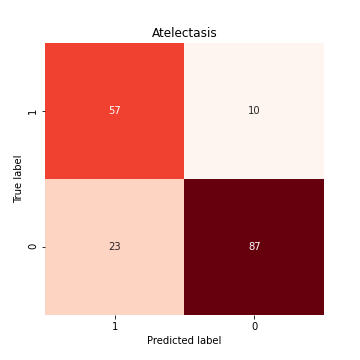
\includegraphics[width=69mm]{Tesi/images/Results/Atelectasis_cf.png} &   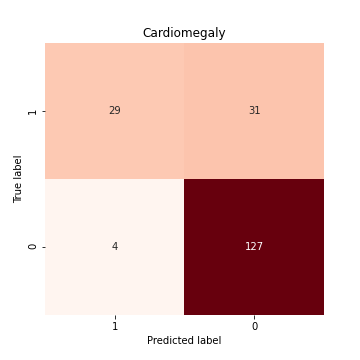
\includegraphics[width=69mm]{Tesi/images/Results/Cardiomegaly_cf.png} \\
\footnotesize{Uncertain: 25} & \footnotesize{Uncertain: 11} \\[6pt]
\multicolumn{2}{c}{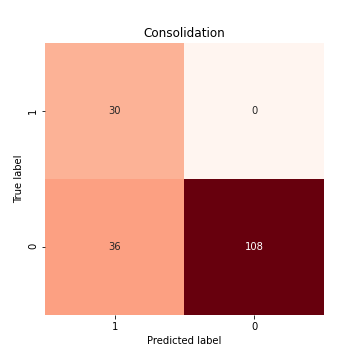
\includegraphics[width=69mm]{Tesi/images/Results/Consolidation_cf.png} }\\
\multicolumn{2}{c}{\footnotesize{Uncertain: 28}}
\end{tabular}
\end{figure}

\begin{figure}[h!]
\begin{tabular}{cc}
  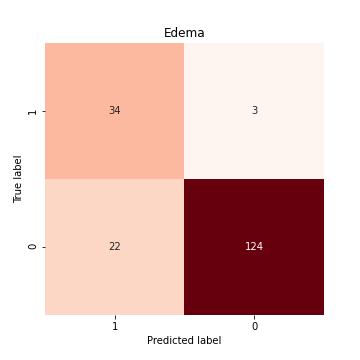
\includegraphics[width=69mm]{Tesi/images/Results/Edema_cf.png} &   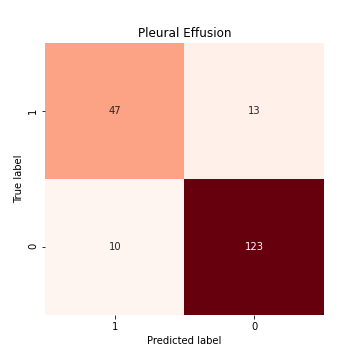
\includegraphics[width=69mm]{Tesi/images/Results/Pleural Effusion_cf.png} \\
\footnotesize{Uncertain: 19} & \footnotesize{Uncertain: 9} \\[6pt]
\end{tabular}
\caption{Confusion Matrices}
\label{fig:figure_5.14}
\end{figure}





\section{Class Activation Map}
\label{sec:cam_results}
We will now show some samples of the Class Activation Maps that have been generated. Differently from previous works, we also provided, together with the \ac{CAM}, a method to automatically extract a bounding box surrounding the area interested by the disease. Given the fact that it's hard to evaluate their goodness without having a medical background, we checked out how the model behaves in localizing the Support Devices, more easily identifiable also by a non expert eye. In Figure \ref{fig:figure_5.15} we can clearly see that the model is able to surround the medical device positioned in patient's chest.

\vspace{10mm}

\begin{figure}[htbp!]
\centering
\begin{tabular}{ccc}
 &\textbf{Support Device}& \\
\vspace{2mm}
  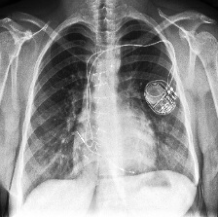
\includegraphics[width=35mm]{Tesi/images/CAMs/CAM2/image.png} &   
  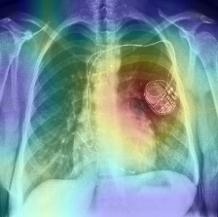
\includegraphics[width=35mm]{Tesi/images/CAMs/CAM2/image_cam.png} &   
  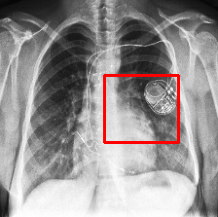
\includegraphics[width=35mm]{Tesi/images/CAMs/CAM2/image_bbox.png} \\
\footnotesize{CXR} & \footnotesize{CAM} & \footnotesize{Bounding Box} \\[6pt]
\end{tabular}
\caption[Support Device CAM-1]{}
\label{fig:figure_5.15}
\end{figure}


\begin{figure}[htbp!]
\centering
\begin{tabular}{ccc}
 &\textbf{Support Device}& \\
\vspace{2mm}
  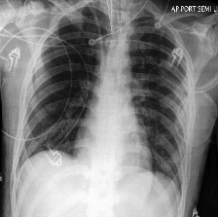
\includegraphics[width=35mm]{Tesi/images/CAMs/CAM1/image.png} &   
  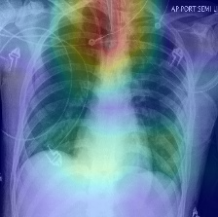
\includegraphics[width=35mm]{Tesi/images/CAMs/CAM1/image_cam.png} &   
  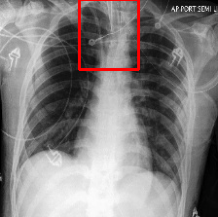
\includegraphics[width=35mm]{Tesi/images/CAMs/CAM1/image_bbox.png} \\
\footnotesize{CXR} & \footnotesize{CAM} & \footnotesize{Bounding Box} \\[6pt]
\end{tabular}
\caption[Support Device CAM-2]{}
\label{fig:figure_5.16}
\end{figure}

\begin{figure}[htbp!]
\centering
\begin{tabular}{ccc}
 &\textbf{Support Device}& \\
\vspace{2mm}
  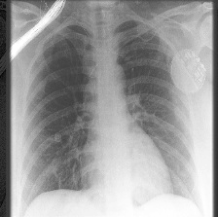
\includegraphics[width=35mm]{Tesi/images/CAMs/CAM3/image.png} &   
  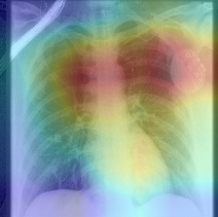
\includegraphics[width=35mm]{Tesi/images/CAMs/CAM3/image_cam.png} &   
  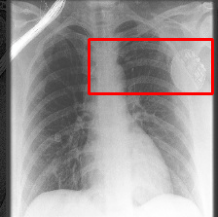
\includegraphics[width=35mm]{Tesi/images/CAMs/CAM3/image_bbox.png} \\
\footnotesize{CXR} & \footnotesize{CAM} & \footnotesize{Bounding Box} \\[6pt]
\end{tabular}
\caption[Support Device CAM-3]{}
\label{fig:figure_5.17}
\end{figure}


\begin{figure}[htbp!]
\centering
\begin{tabular}{ccc}
 &\textbf{Atelectasis}& \\
\vspace{2mm}
  \includegraphics[width=35mm]{Tesi/images/CAMs/CAM4/image.png} &   
  \includegraphics[width=35mm]{Tesi/images/CAMs/CAM4/image_cam.png} &   
  \includegraphics[width=35mm]{Tesi/images/CAMs/CAM4/image_bbox.png} \\
\footnotesize{CXR} & \footnotesize{CAM} & \footnotesize{Bounding Box} \\[6pt]
\end{tabular}
\caption[Atelectasis CAM-1]{}
\label{fig:figure_5.18}
\end{figure}

\begin{figure}[htbp!]
\centering
\begin{tabular}{ccc}
 &\textbf{Atelectasis}& \\
\vspace{2mm}
  \includegraphics[width=35mm]{Tesi/images/CAMs/CAM5/image.png} &   
  \includegraphics[width=35mm]{Tesi/images/CAMs/CAM5/image_cam.png} &   
  \includegraphics[width=35mm]{Tesi/images/CAMs/CAM5/image_bbox.png} \\
\footnotesize{CXR} & \footnotesize{CAM} & \footnotesize{Bounding Box} \\[6pt]
\end{tabular}
\caption[Atelectasis CAM-2]{}
\label{fig:figure_5.19}
\end{figure}


\begin{figure}[htbp!]
\centering
\begin{tabular}{ccc}
 &\textbf{Cardiomegaly}& \\
\vspace{2mm}
  \includegraphics[width=35mm]{Tesi/images/CAMs/CAM6/image.png} &   
  \includegraphics[width=35mm]{Tesi/images/CAMs/CAM6/image_cam.png} &   
  \includegraphics[width=35mm]{Tesi/images/CAMs/CAM6/image_bbox.png} \\
\footnotesize{CXR} & \footnotesize{CAM} & \footnotesize{Bounding Box} \\[6pt]
\end{tabular}
\caption[Cadiomegaly CAM-1]{}
\label{fig:figure_5.20}
\end{figure}

\begin{figure}[htbp!]
\centering
\begin{tabular}{ccc}
 &\textbf{Cardiomegaly}& \\
\vspace{2mm}
  \includegraphics[width=35mm]{Tesi/images/CAMs/CAM7/image.png} &   
  \includegraphics[width=35mm]{Tesi/images/CAMs/CAM7/image_cam.png} &   
  \includegraphics[width=35mm]{Tesi/images/CAMs/CAM7/image_bbox.png} \\
\footnotesize{CXR} & \footnotesize{CAM} & \footnotesize{Bounding Box} \\[6pt]
\end{tabular}
\caption[Cadiomegaly CAM-2]{}
\label{fig:figure_5.21}
\end{figure}


\begin{figure}[htbp!]
\centering
\begin{tabular}{ccc}
 &\textbf{Consolidation}& \\
\vspace{2mm}
  \includegraphics[width=35mm]{Tesi/images/CAMs/CAM8/image.png} &   
  \includegraphics[width=35mm]{Tesi/images/CAMs/CAM8/image_cam.png} &   
  \includegraphics[width=35mm]{Tesi/images/CAMs/CAM8/image_bbox.png} \\
\footnotesize{CXR} & \footnotesize{CAM} & \footnotesize{Bounding Box} \\[6pt]
\end{tabular}
\caption[Consolidation CAM-1]{}
\label{fig:figure_5.22}
\end{figure}

\newpage

\begin{figure}[htbp!]
\centering
\begin{tabular}{ccc}
 &\textbf{Consolidation}& \\
\vspace{2mm}
  \includegraphics[width=35mm]{Tesi/images/CAMs/CAM9/image.png} &   
  \includegraphics[width=35mm]{Tesi/images/CAMs/CAM9/image_cam.png} &   
  \includegraphics[width=35mm]{Tesi/images/CAMs/CAM9/image_bbox.png} \\
\footnotesize{CXR} & \footnotesize{CAM} & \footnotesize{Bounding Box} \\[6pt]
\end{tabular}
\caption[Consolidation CAM-2]{}
\label{fig:figure_5.23}
\end{figure}

\begin{figure}[htbp!]
\centering
\begin{tabular}{ccc}
 &\textbf{Edema}& \\
\vspace{2mm}
  \includegraphics[width=35mm]{Tesi/images/CAMs/CAM10/image.png} &   
  \includegraphics[width=35mm]{Tesi/images/CAMs/CAM10/image_cam.png} &   
  \includegraphics[width=35mm]{Tesi/images/CAMs/CAM10/image_bbox.png} \\
\footnotesize{CXR} & \footnotesize{CAM} & \footnotesize{Bounding Box} \\[6pt]
\end{tabular}
\caption[Edema CAM-1]{}
\label{fig:figure_5.24}
\end{figure}



\begin{figure}[htbp!]
\centering
\begin{tabular}{ccc}
 &\textbf{Edema}& \\
\vspace{2mm}
  \includegraphics[width=35mm]{Tesi/images/CAMs/CAM11/image.png} &   
  \includegraphics[width=35mm]{Tesi/images/CAMs/CAM11/image_cam.png} &   
  \includegraphics[width=35mm]{Tesi/images/CAMs/CAM11/image_bbox.png} \\
\footnotesize{CXR} & \footnotesize{CAM} & \footnotesize{Bounding Box} \\[6pt]
\end{tabular}
\caption[Edema CAM-2]{}
\label{fig:figure_5.25}
\end{figure}

\newpage

\begin{figure}[htbp!]
\centering
\begin{tabular}{ccc}
 &\textbf{Pleural Effusion}& \\
\vspace{2mm}
  \includegraphics[width=35mm]{Tesi/images/CAMs/CAM12/image.png} &   
  \includegraphics[width=35mm]{Tesi/images/CAMs/CAM12/image_cam.png} &   
  \includegraphics[width=35mm]{Tesi/images/CAMs/CAM12/image_bbox.png} \\
\footnotesize{CXR} & \footnotesize{CAM} & \footnotesize{Bounding Box} \\[6pt]
\end{tabular}
\caption[Pleural Effusion CAM-1]{}
\label{fig:figure_5.26}
\end{figure}

\begin{figure}[htbp!]
\centering
\begin{tabular}{ccc}
 &\textbf{Pleural Effusion}& \\
\vspace{2mm}
  \includegraphics[width=35mm]{Tesi/images/CAMs/CAM13/image.png} &   
  \includegraphics[width=35mm]{Tesi/images/CAMs/CAM13/image_cam.png} &   
  \includegraphics[width=35mm]{Tesi/images/CAMs/CAM13/image_bbox.png} \\
\footnotesize{CXR} & \footnotesize{CAM} & \footnotesize{Bounding Box} \\[6pt]
\end{tabular}
\caption[Pleural Effusion CAM-2]{}
\label{fig:figure_5.27}
\end{figure}



\section{Summary}
\label{sec:chapter_5_summary}
At the beginning of this chapter we have presented the evaluation criteria we have used to assess the performance of our models. Then we have presented all the results we achieved using the approaches defined in the previous chapters, discussing them and comparing each other. Using the confusion matrices we tried to give the lecturer a more comprehensible summary about our model performances. We then compared our results with that obtained by the state of the art. Finally, we have provided some samples of the \acp{CAM} and Bounding Boxes that have been generated. In the next chapter we will give some considerations about our overall work and we will discuss some possible future works related to it.

% Conclusioni
\chapter{Conclusions And Future Works}
\label{cha:conclusions}

In this chapter we will conclude our work, giving some general considerations about what we have done and some possible future works. 

\section{Conclusions}
\label{sec:conclusions}
In this work we have presented the problem of analyzing Chest X-Rays to automatically classify some pathologies. Starting from some works that were previously carried out by the scientific community, we developed a system able to achieve a mean AUROC across five different diseases of 0.902. Although Pham et al. \cite{pham2019interpreting} in their work obtained a better result, we introduced some novelties. 

\vspace{5mm}

Starting from the techniques proposed by the related works mentioned above, we developed multiple models using U-Ones and Label Smooth Regularization to deal with uncertain labels and Conditional Training to exploit diseases hierarchy. Then we investigated different approaches to aggregate the different models, showing that, instead of making a simple average of the predictions, the use of a weighted average, based on models' entropy, can improve the ensemble performance. Then, using the embeddings extracted by means of the \acp{CNN}, we showed that is possible, taking less time and computational resources, to build a system able to reach (or even surpass) the performance obtained by neural networks. Then, using the confusion matrices we tried, differently from other works, to give a more comprehensible vision of our model's output, showing exactly the number of correct and incorrect predictions, allowing also the system to abstain in case it is very uncertain about its diagnosis. 
Finally, for what it concern the pathologies visualization, we tried to improve it by aggregating the different Class Activation Maps produced by the models and we proposed a system to automatically extract a bounding box surrounding the region that most probably is interested by the disease. 

\section{Future Works}
\label{sec:future_works}
We will now talk about some approaches that could be investigated to improve this work.


\vspace{5mm}

In our research we tried to build a model that was as general as possible. However Pham et al. \cite{pham2019interpreting}, in their work, used some performance tweaking that allow their model to achieve very high results, with the downside of losing some generalization capability. It could be interesting to check whether those performance tweaking would actually lead to a better result or not.

\vspace{5mm}
For what it concern data, as we already said in Chapter \ref{cha:third_chapter}, during the preprocessing we discarded some informations related to the patients, such as its age and gender. These data instead, could be leveraged, trying to check if, giving them as additional input to a model, is possible to enhance the predictions. 
Moreover, in our work we only employed the frontal CXR, but the dataset we used comes with a pretty large number of Lateral CXR. A system able to process both a Frontal and a Lateral view would probably be able to better discriminate among the different diseases. 

\vspace{5mm}

Moreover, as we have seen, one of the biggest issues related to Chexpert dataset is that it's quite unbalanced, causing the perfomance of the less represented class to be worse than the other. Using some class balancing algorithm could produce an overall improvement.
For what it concern data, finally, it is worth noting that it exist a dataset whose \acp{CXR} have been labelled using the same approach employed in Chexpert \cite{johnson2019mimiccxrjpg}, containing almost 370 thousand additional images that could be used to train the models (with the downside that this approach requires more time and computational resources)

\vspace{5mm}

As we already told, the embeddings are able to capture the meaningful information needed to identify the presence or absence of a disease, with the advantage of drastically reducing the input dimension. In our work we used them to train Random Forest and XGBoost. However, given the small dimension of the embeddings (compared to that of the original images), it would be possible to investigate any other Machine Learning algorithm, even those that initially seemed to be not suitable for solving the task of CXR image analysis.

\vspace{5mm}

Once the embeddings have been extracted, moreover, they could be used to train models able to find any other pathology, not only those present in CheXpert. As proof of concept, we used them to identify the Chest X-Rays affected by SARS-CoV-2, the virus causing a pandemic that, starting from December 2019, spread all over the world. Using our trained \acp{CNN}, we extracted the embeddings of almost one hundred \acp{CXR} coming from sick patients and we used them to train a binary classifier using XGBoost, with the aim of distinguishing a regular Pneumonia (whose corresponding \acp{CXR} were already provided by CheXpert) from one caused by SARS-CoV-2. We used 10-fold cross validation as evaluation approach, obtaining the results in Table \ref{table:table_6.1}.

\vspace{5mm}

\begin{table}[h!]
\centering
\begin{tabular}{|l|l|l|} 
\hline
\textbf{Fold} & \textbf{Accuracy} & \textbf{AUROC} \\
\hline
Fold-1  &1.000 & 1.000\\ \hline
Fold-2  &0.947 & 0.929\\ \hline
Fold-3  &0.947 & 0.955\\\hline
Fold-4  &1.000 & 1.000\\\hline
Fold-5  &0.947 & 0.944\\\hline
Fold-6  &0.947 & 0.944\\\hline
Fold-7  &0.895 & 0.889\\\hline
Fold-8  &1.000 & 1.000\\\hline
Fold-9  &0.947 & 0.944\\\hline
Fold-10 &1.000 & 1.000\\\hline

\rowcolor[rgb]{0.851,0.851,0.851}AVG & 0.963 & 0.961\\
\hline
\end{tabular}

\caption[COVID-19 results]{COVID-19 Accuracy and AUROC of the 10 folds.}
\label{table:table_6.1}
\end{table}

\vspace{3mm}

As we can see, we obtained an average AUROC of 0.961 without using the full images, but exploiting only the embeddings. In some cases the model is able to perfectly distinguish the two diseases, as we can see in the confusion matrix reported \ref{fig:figure_6.1}.

\vspace{5mm}

\begin{figure}[htbp!]
\centering
\includegraphics[scale=0.62]{Tesi/images/COVID CM.png}
\caption{COVID-19 Confusion Matrix}
\label{fig:figure_6.1}
\end{figure}

\newpage
\vspace{5mm}
Finally, the last approach we want to propose is that of using the bounding box that we generated to extract the area interested by the pathology and use it as input to the model, in order to let it focus its attention on a smaller region of the image.




% Appendici

%\renewcommand{\chaptermark}[1]{\markboth{\appendixname\ \thechapter.\ #1}{}} % modifica l'intestazione con il nome/lettera dell'appendice
%\fancyhead[LE,RO]{\leftmark}

%\appendix % trasforma i numeri in lettere per fare l'appendice
%\input{chapters/first_appendix}

%\newcommand\blankpage{%
%    \null
%    \thispagestyle{empty}%
%    \addtocounter{page}{+0}%
%    \newpage}

%\afterpage{\blankpage}
% Acronimi
\clearpage\null\thispagestyle{empty}

\chapter*{Acronyms}
\label{cha:acronyms}
\addcontentsline{toc}{chapter}{Acronyms}
\onehalfspacing
\begin{acronym}[\qquad \qquad \qquad \quad]
\acro{AI}{Artificial Intelligence}
\acro{AUROC}{Area Under Receiving Operating Characteristic}
\acro{ANN}{Artificial Neural Network}
\acro{CAM}{Class Activation Map}
\acro{CNN}{Convolutional Neural Network}
\acro{CXR}{Chest X-Ray}
\acro{DL}{Deep Learning}
\acro{FC}{Fully Connected}
\acro{FCNN}{Fully Connected Neural Network}
\acro{FN}{False Negative}
\acro{FP}{False Positive}
\acro{FPR}{False Positive Rate}
\acro{GAP}{Global Average Pooling}
\acro{LSR}{Label Smoothing Regularization}
\acro{ML}{Machine Learning}
\acro{NLP}{Natural Language Processing}
\acro{RF}{Random Forest}
\acro{TN}{True Negative}
\acro{TP}{True Positive}
\acro{TPR}{True Positive Rate}
\end{acronym}


% modifica intestazione della bibliografia
\fancyhead[LE,RO]{\nouppercase{\leftmark}} % cancella il tutto maiuscolo


\appto{\bibsetup}{\raggedright}
% bibliografia
\printbibliography[heading=bibintoc]



\end{document}